% Chapter Template
%!TEX root=../main.tex
\chapter{2-D Memristor Simulation} % Main chapter title

\label{Chapter7} % Change X to a consecutive number; for referencing this chapter elsewhere, use \ref{ChapterX}

\lhead{Chapter 7. \emph{Memristor Simulation}} % Change X to a consecutive number; this is for the header on each page - perhaps a shortened title
\begin{doublespace}

Even though 1-D simulation is able to capture the main characteristics of the memristor it is still lacking certain physical effects that can be captured in a 2-D simulation such as the movement of ions inside the electrolytic solution which cancels some of the applied electric field. This chapter shows the simulation of a memristor in 2-D and compares the results with 1-D simulations. It starts with the simulation of a memristor with different PEDOT:PSS layer thicknesses and shows the changes in particle the density distributions, electric field and current density. Transient simulations with a potential pulse train and a sinusoidal potential are presented and compared to 1-D simulations. Finally current vs time and I-V curves for an actual memristor are used to show the accuracy of 2-D simulations in capturing the behavior of the actual device .  

\section{Effect of PEDOT:PSS Thickness}

The physical dimensions of the memristor \tjsr{is}{are} presented in the previous chapter. The thickness of the PEDOT:PSS layer is very small compared to the other dimensions of the device such as the thickness of the electrolyte and length of the conductive material. This complicates the simulation of the PEDOT:PSS strip using a uniform mesh. Although non uniform meshing seems like an appropriate solution for this problem, a close examination of the numerical limitations show that this is not the case. Decreasing the mesh size in one dimension severely reduces the maximum time step for the entire simulation therefore non uniform meshing is not feasible for this problem. 

An alternative solution to the meshing problem is \tjsr{using}{embedding} an infinitesimally thin PEDOT:PSS layer in a 2-D simulation. This method is used for the memristor simulations in this chapter. For PEDOT:PSS, the effects in 2-D are ignored since the layer thickness is 10000 times smaller than other dimensions such as the thickness of the electrolyte. For the holes in the conductive layer only the horizontal component of the electric field is used and all the current densities are calculated in 1-D. Following plots compare two simulations with PEDOT:PSS thicknesses higher than the actual device thickness and a 2-D simulation with a 1-D PEDOT:PSS layer.  

\begin{figure}[!htp]
\centering
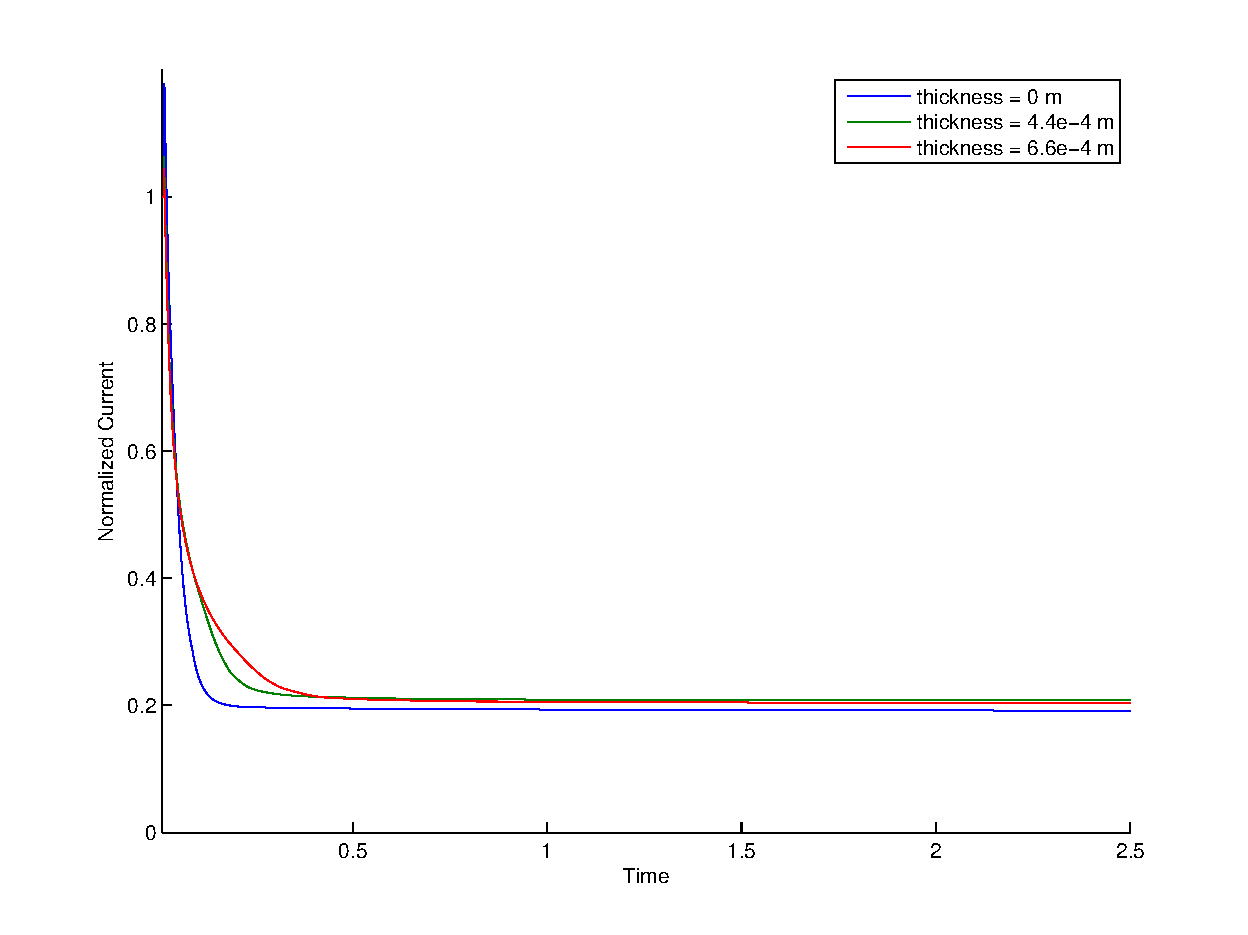
\includegraphics[scale=0.55]{2D_Memristor_Thick_Resistivity}
\caption{Normalized current over time or different PEDOT:PSS thicknesses} 
\label{thick_resistivity}
\end{figure}

The memristor is simulated using a constant potential at the contacts. \tjs{The} left metal contact is \tjs{at} 1 V and the right metal contact is grounded. The current density measured at the right contact for different PEDOT:PSS thicknesses is shown in figure \ref{thick_resistivity}. These plots show that as the PEDOT:PSS thickness gets smaller the device responds faster. This is due to the decrease \tjs{[Is distance correct or is the larger volume??]} in the distance lithium ions have to travel inside PEDOT:PSS in order to change its resistivity. Another change in the behavior of the memristor is its resistivity at steady state. The increase in resistivity for different PEDOT:PSS thicknesses at steady state can be attributed to the ion/hole interaction at the interface between the PEDOT:PSS and the electrolyte solution which is illustrated in the following figures \ref{thick_p_ss}, \ref{thick_li_ss} and \ref{thick_perch_ss}.

\begin{figure}[!htp]
\centering
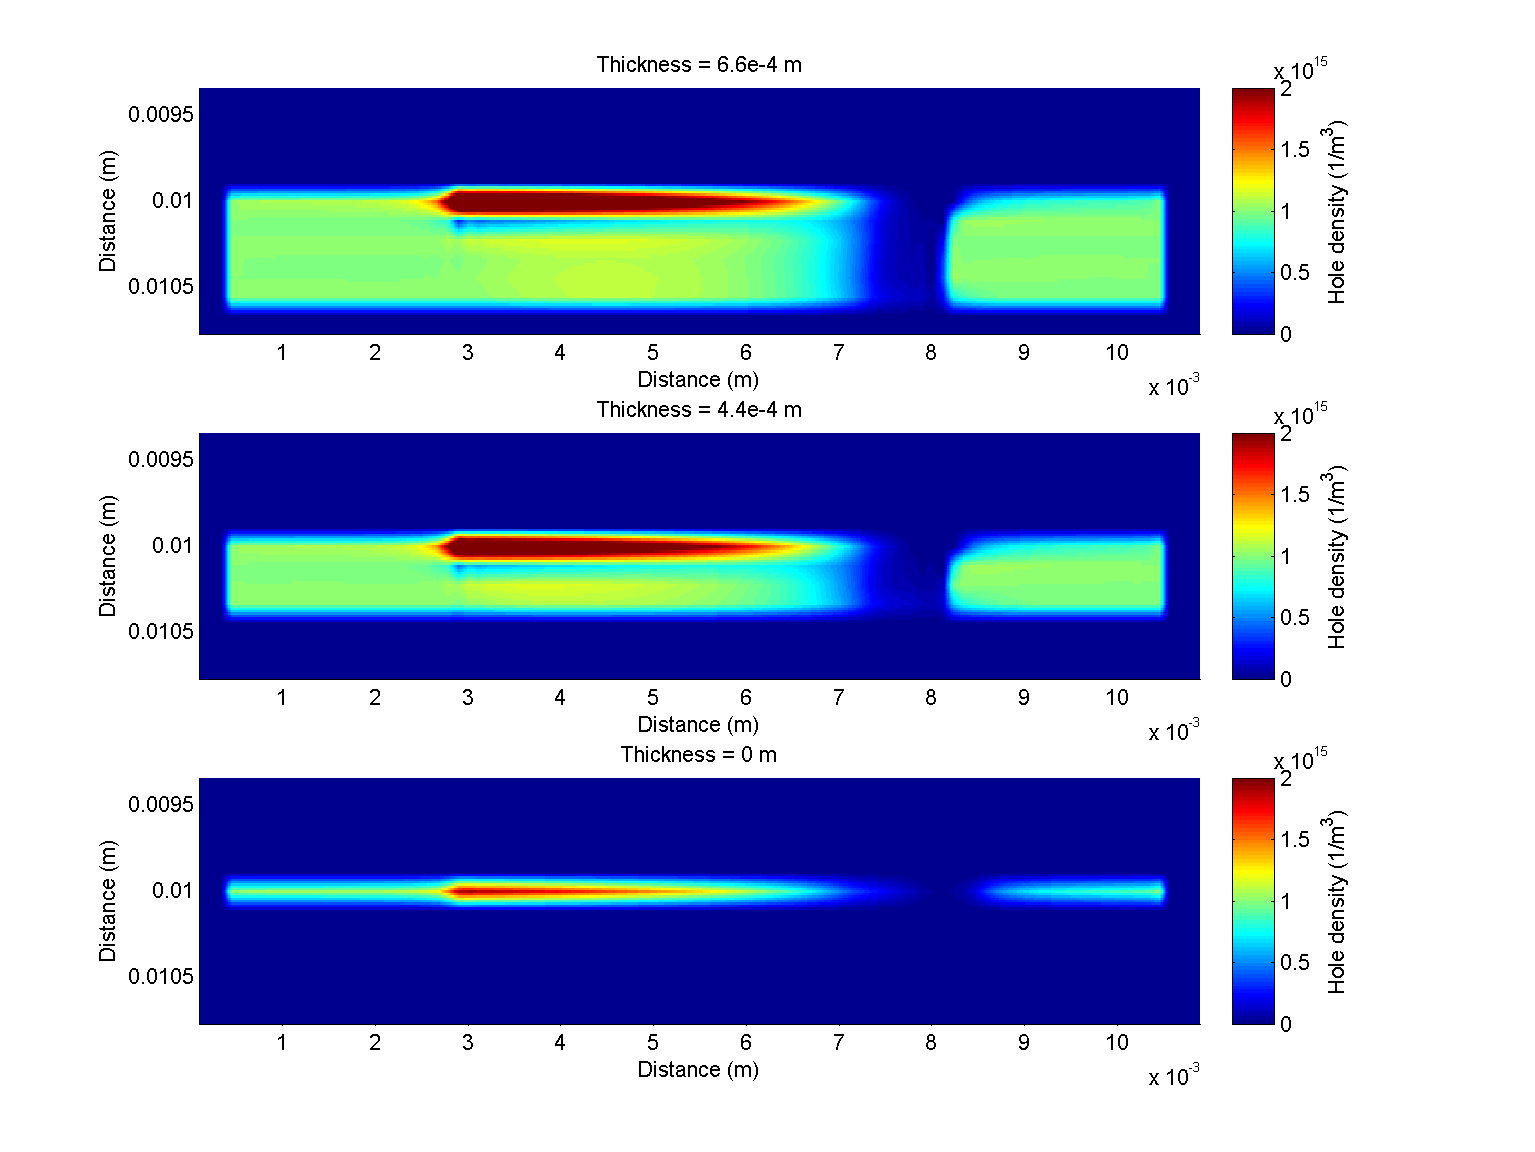
\includegraphics[scale=0.50]{2D_Memristor_Thick_Hole_SS}
\caption{Hole distribution at steady state for different PEDOT:PSS thicknesses} 
\label{thick_p_ss}
\end{figure}

Figure \ref{thick_p_ss} shows the hole distribution in PEDOT:PSS at steady state for different thicknesses. The electrolyte is on top of PEDOT:PSS but it is not visible in these plots since its hole density is zero at all times. As lithium ions move into the PEDOT:PSS they move towards the metal contact and accumulate at the wet/dry interface. There is a lack of holes around the region where lithium ions accumulate. This effect can be seen in figures \ref{thick_p_ss} and  \ref{thick_li_ss}. For all the plots, there is a section of the hole distribution which is missing due to high concentration of lithium ions.

\begin{figure}[!htp]
\centering
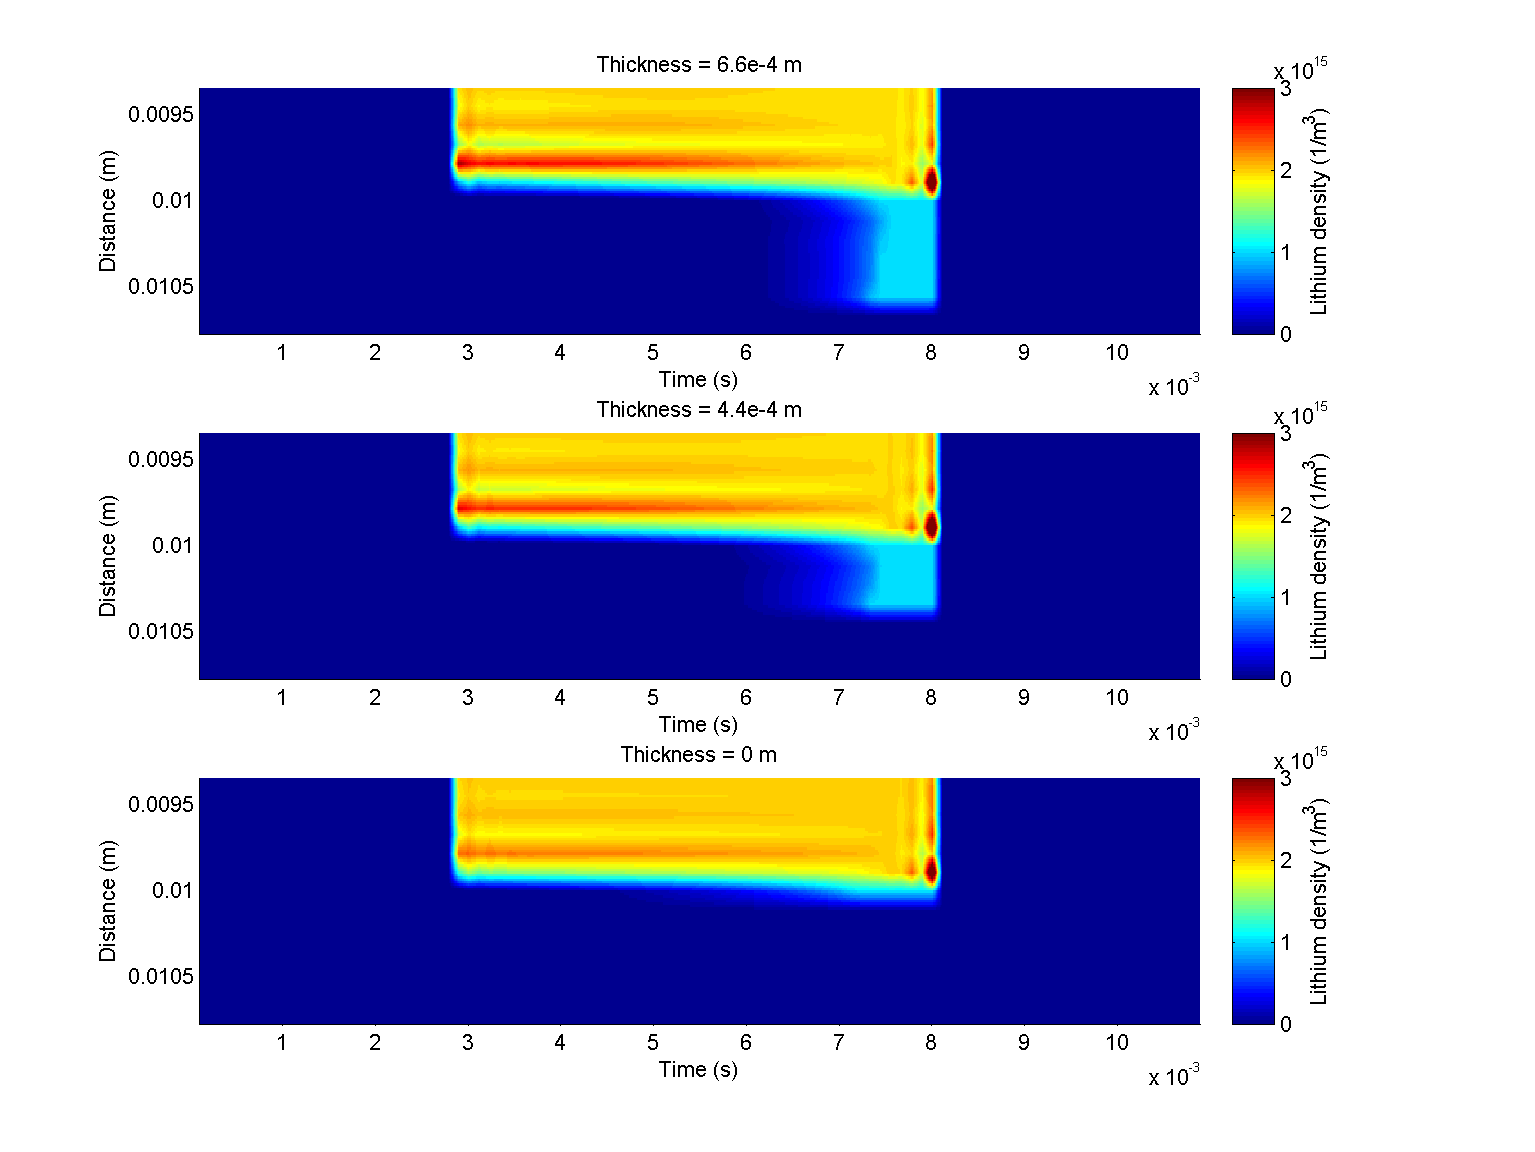
\includegraphics[scale=0.50]{2D_Memristor_Thick_Lithium_SS}
\caption{Lithium distribution at steady state for different PEDOT:PSS thicknesses} 
\label{thick_li_ss}
\end{figure}

The accumulation of holes at the surface of the PEDOT:PSS is due to the perchlorate accumulation near the positive contact in the electrolyte (figure \ref{thick_perch_ss}). As perchlorate ions accumulate on the surface of the PEDOT:PSS they also attract holes towards the surface.

\begin{figure}[!htp]
\centering
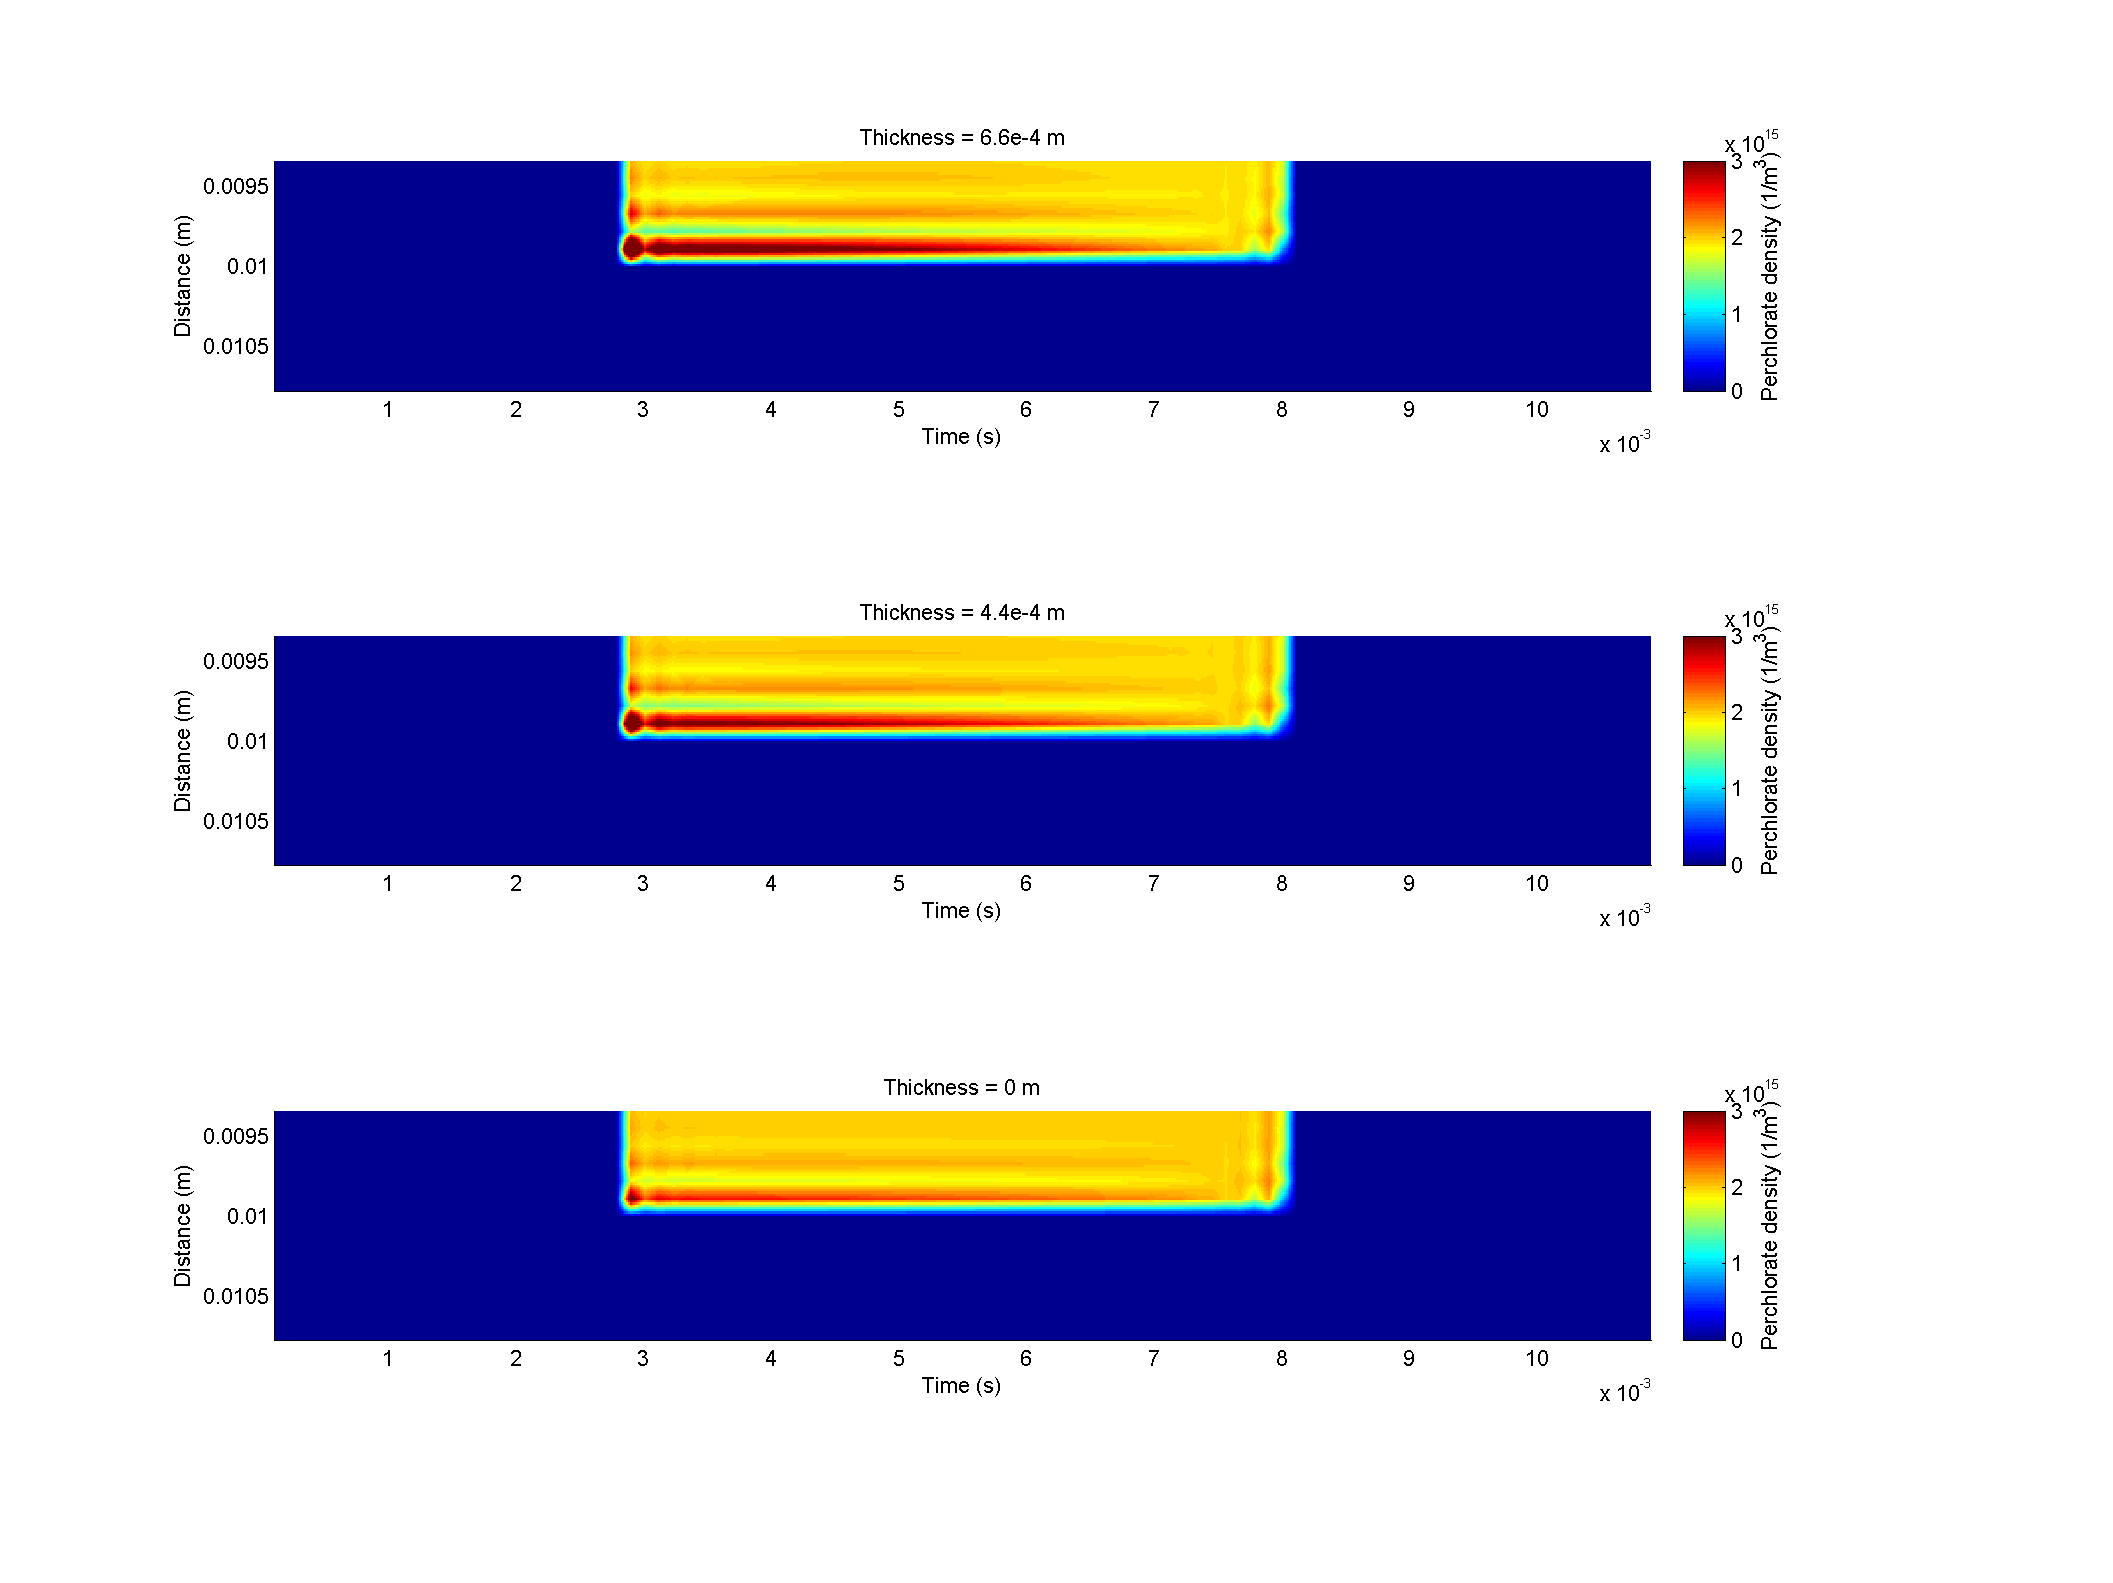
\includegraphics[scale=0.40]{2D_Memristor_Thick_Perchlorate_SS}
\caption{Perchlorate distribution at steady state for different PEDOT:PSS thicknesses} 
\label{thick_perch_ss}
\end{figure}

Figure \ref{thick_netq_p} shows the charge density of holes at the surface of the PEDOT:PSS and the net charge density in the electrolyte near PEDOT:PSS. Negative charges that accumulate on the left side of the electrolyte create\tjsr{s}{} an abundance of holes where\tjs{as} positive charges on the right side creates a lack of holes. This additional mechanism is the key difference between 1-D and 2-D simulations. In 1-D simulation, ion density inside the electrolyte and the changes in the electric field due to these charges were not present.

\begin{figure}[!htp] 
\centering
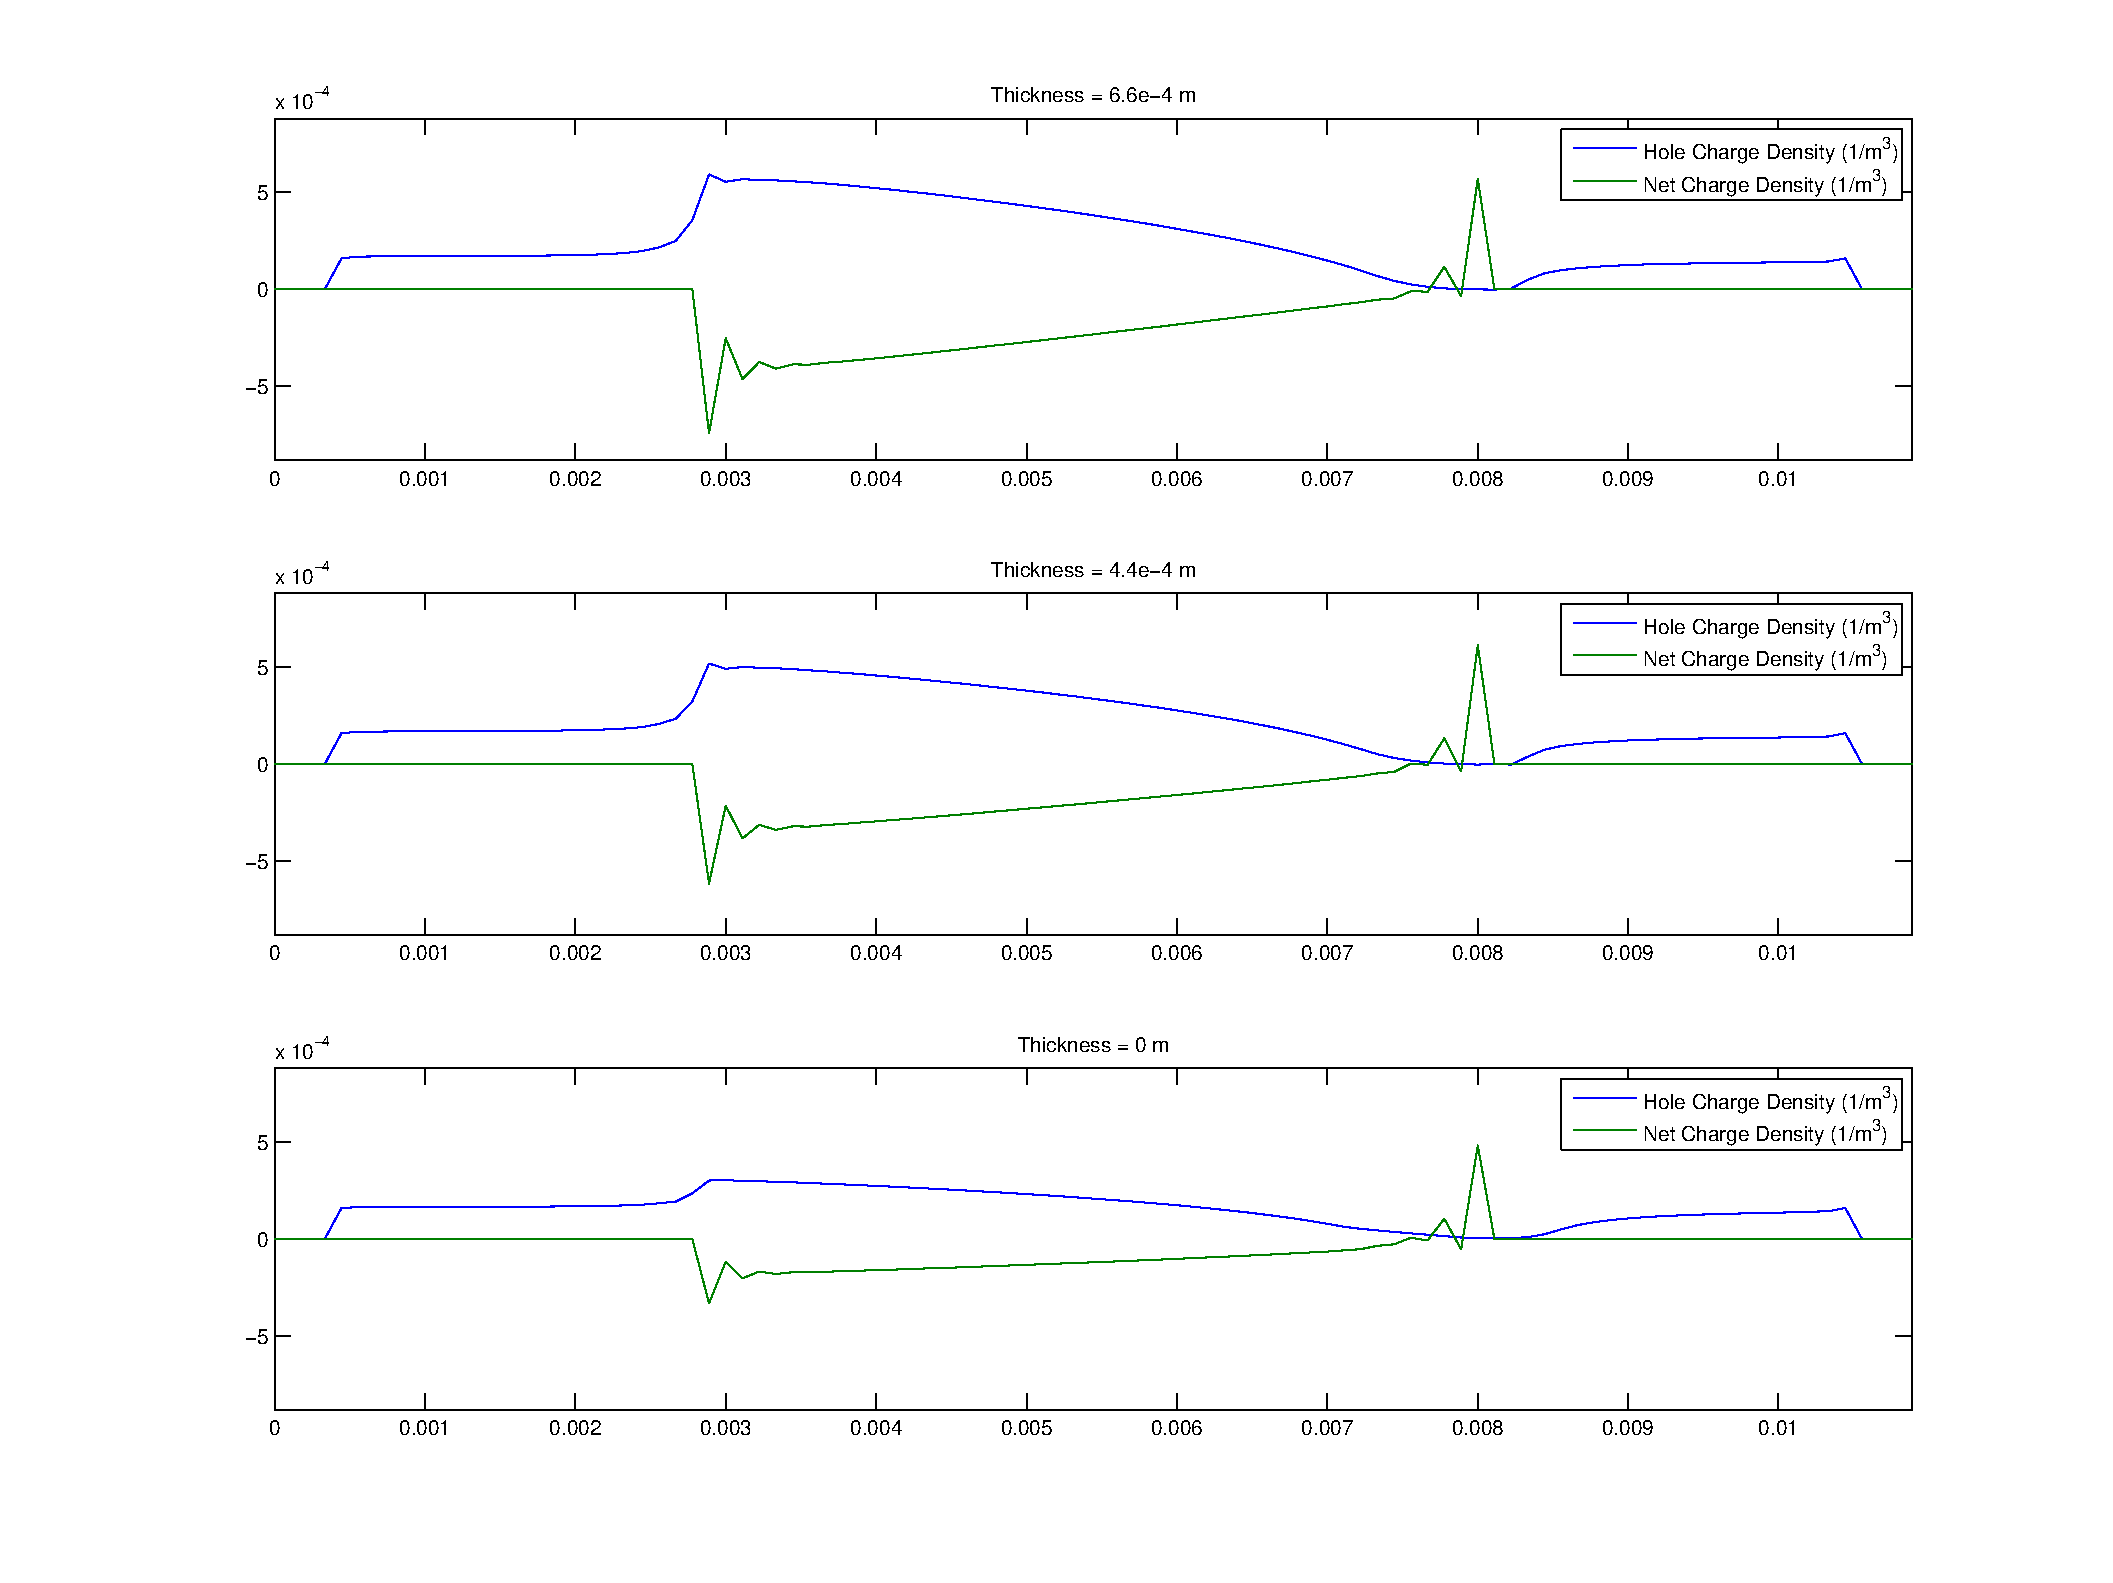
\includegraphics[scale=0.40]{2D_Memristor_netq_hole}
\caption{Net charge distribution at steady state for different PEDOT:PSS thicknesses} 
\label{thick_netq_p}
\end{figure}

As shown in the previous chapter, the electric field has the highest value where the lithium ions accumulate. The figure \ref{thick_efield} shows the change in the shape of the electric field as PEDOT:PSS gets thinner. For all the plots most of the potential drop occurs where lithium ions accumulate and it is concentrated at the surface of the PEDOT:PSS. 

The above plots show that changing the thickness of the PEDOT:PSS does not have a drastic effect in the operation of the memristor since most of the changes occur at the interface between electrolyte and PEDOT:PSS. \tjs{A} 1-D approximation of the polymer conductor contains all the necessary physics for the simulation of the memristor described in chapter 5.

\begin{figure}[!htp]
\centering
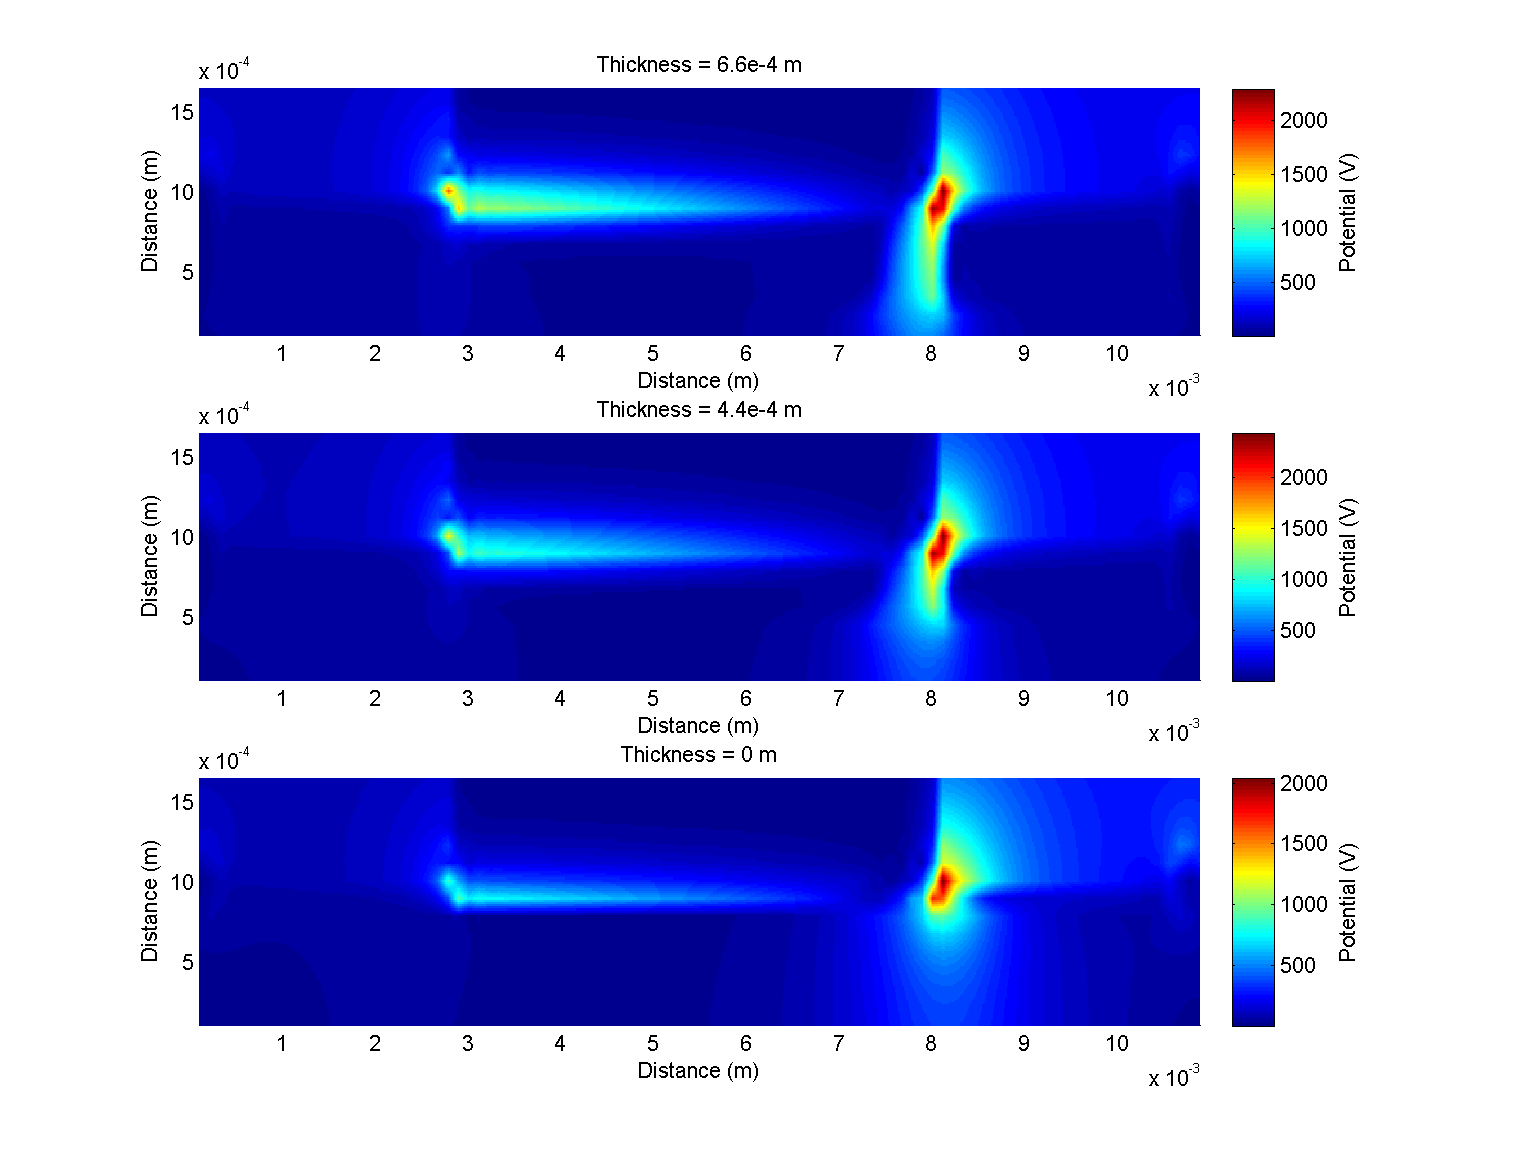
\includegraphics[scale=0.50]{2D_Memristor_Thick_E}
\caption{Electric field strength at steady state for different PEDOT:PSS thicknesses} 
\label{thick_efield}
\end{figure}


\clearpage
\section{2-D Memristor Simulation Using a Potential Pulse Train}

\tjs{The} following results are generated using the same boundary and initial conditions as the simulations in the previous section in order to show the differences between 1-D and 2-D memristor models.

\begin{figure}[!htp]
\centering
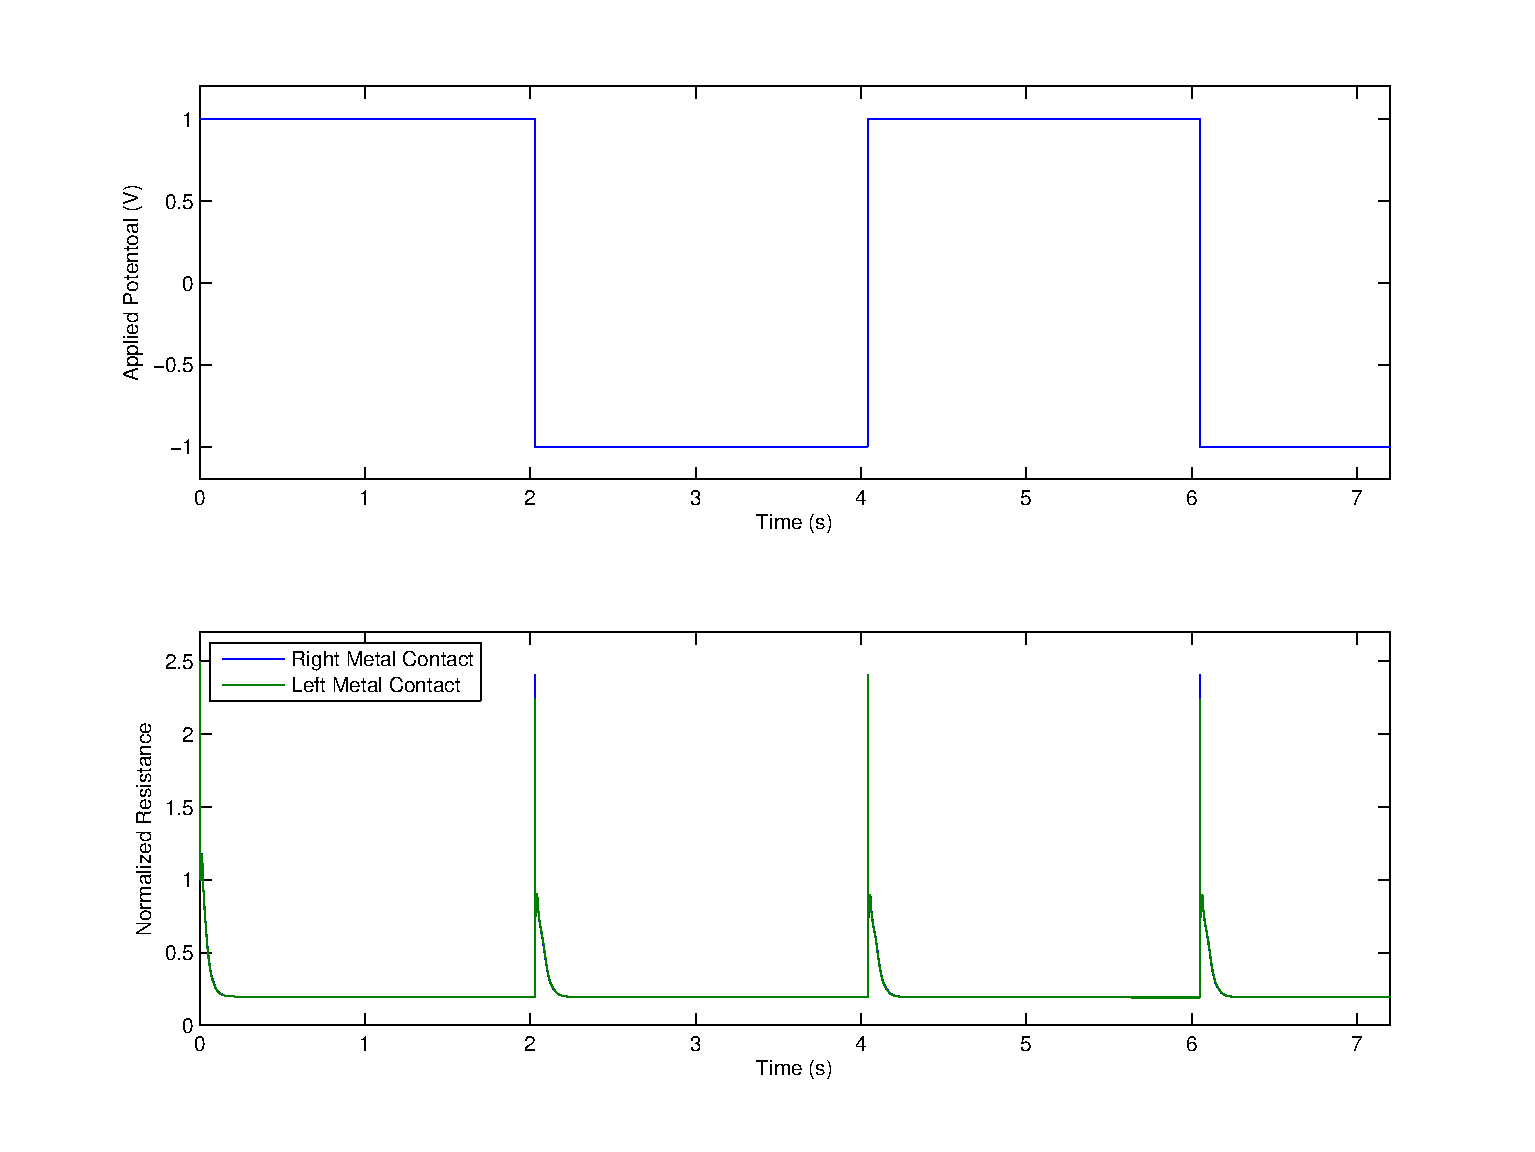
\includegraphics[scale=0.50]{2D_Memristor_Pulse_Train}
\caption{Applied potential and normalized current over time of a 2-D memristor} 
\label{2D_mem_train}
\end{figure}

 Even though the general trend of the current densities are similar for the plots (\ref{MemResTrain} and \ref{2D_mem_train}), there are some essential differences between 1-D and 2-D simulations. The movement of the lithium ions controls the change in the resistivity over time therefore the response of the device is dependent on the velocity of the lithium ions which is a function of mobility and the electric field. In 1-D simulations the vertical mobility of the lithium needs to be adjusted in order to account for the thickness of the electrolyte since it is collapsed into a single layer for 1-D simulations. Because of this the mobility of the lithium has different values in different directions. Additionally the strength of the electric field is not constant over the entire PEDOT:PSS strip. The speed of the lithium ions vary depending on their position and direction due to the changes in the mobility and the electric field.
 
The amount of charge that can accumulate inside the PEDOT:PSS is dependent on the drift and the diffusion of the lithium ions. Due to the electric field, the lithium ions are forced to accumulate on one side of the PEDOT:PSS layer instead of being evenly distributed. The ratio of vertical to horizontal drift of the lithium near the metal contact determines the maximum amount of charge that can accumulate which determines the maximum resistivity of the material. The results of both simulations show that the relative strength of the lithium drift current from the electrolyte to the PEDOT:PSS compared to the drift from one contact to the other is greater in 1-D simulation. This explains why the current density at steady state is lower in 2-D memristor simulations. 

\begin{figure}[!htp]
\centering
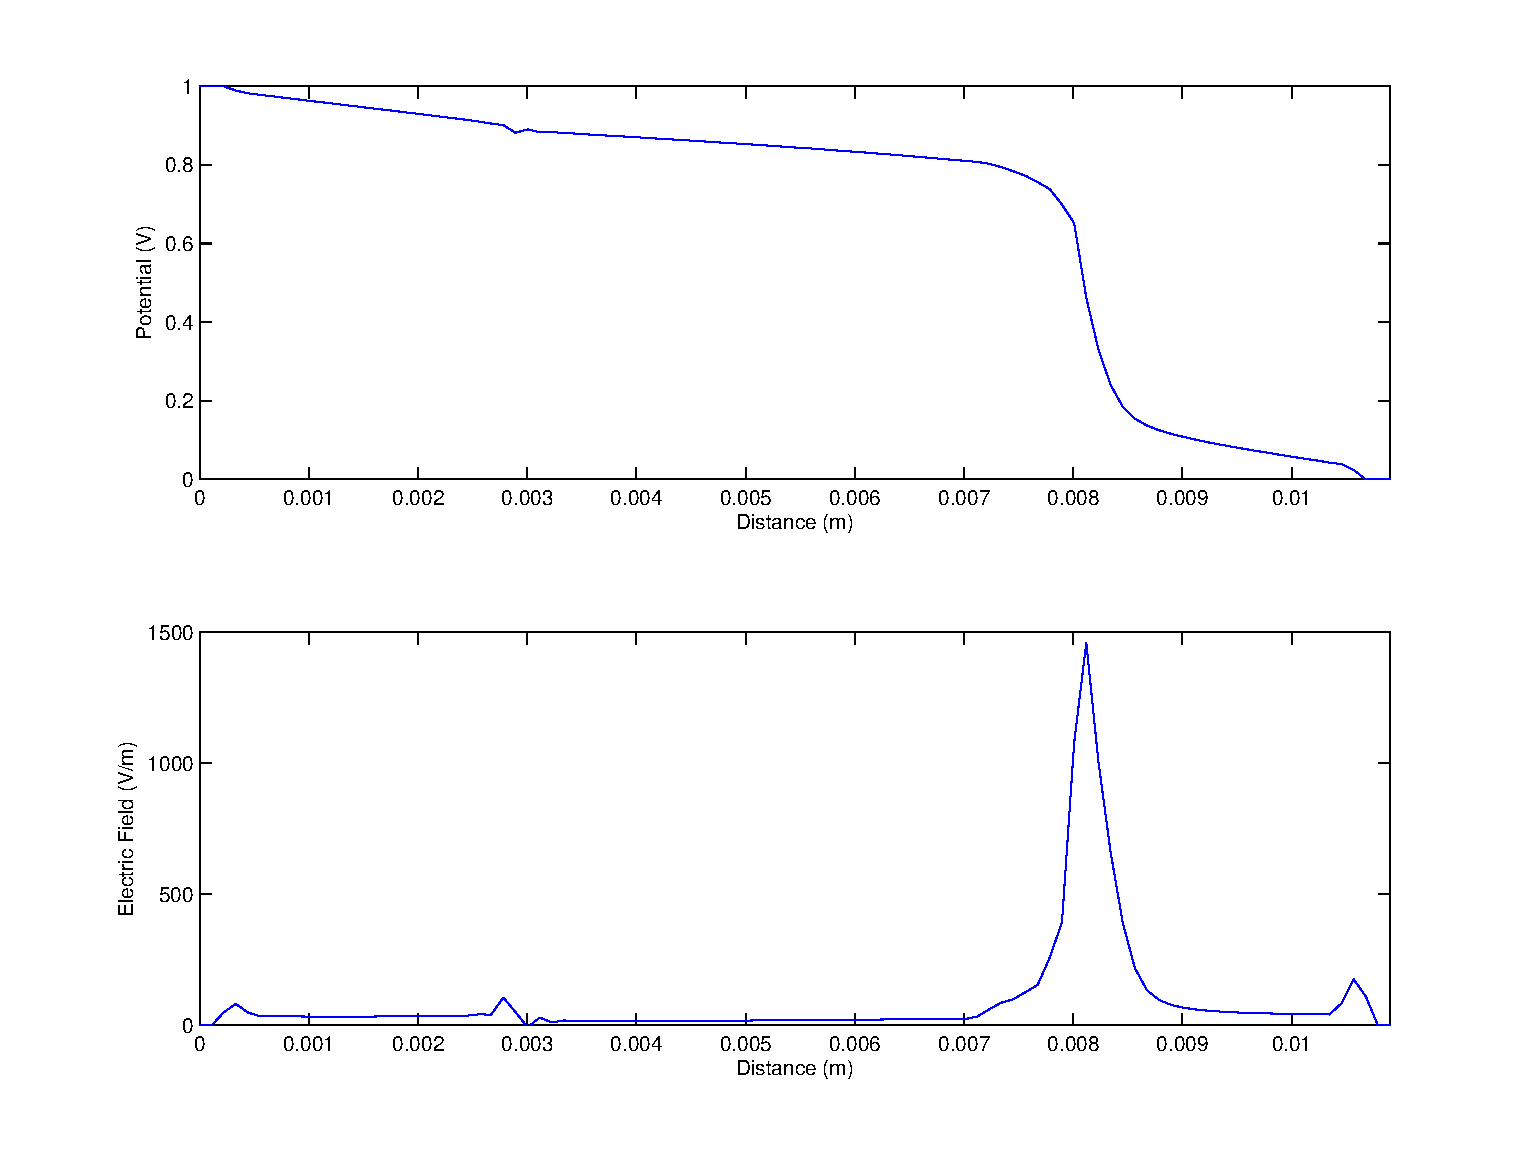
\includegraphics[scale=0.50]{2D_Memristor_Pulse_Train_EV}
\caption{Electric field and potential at steady state along PEDOT:PSS} 
\label{2D_E_V_ss}
\end{figure}

Electric field and potential distributions (figure \ref{2D_E_V_ss}) for 1-D and 2-D simulations are almost identical at steady state. In both cases most of the potential drop and electric field occurs where lithium ions accumulate.

The lithium and hole density plots shown in figure \ref{lit_hole_dist} are also similar to the plots (\ref{MempLi}) shown in section 6.4.1. For both of the simulations the lithium ions move into the PEDOT:PSS until the end of the wet region. At the same time holes move out of the wet/dry interface and create a high resistance region.

\begin{figure}[!htp]
\centering
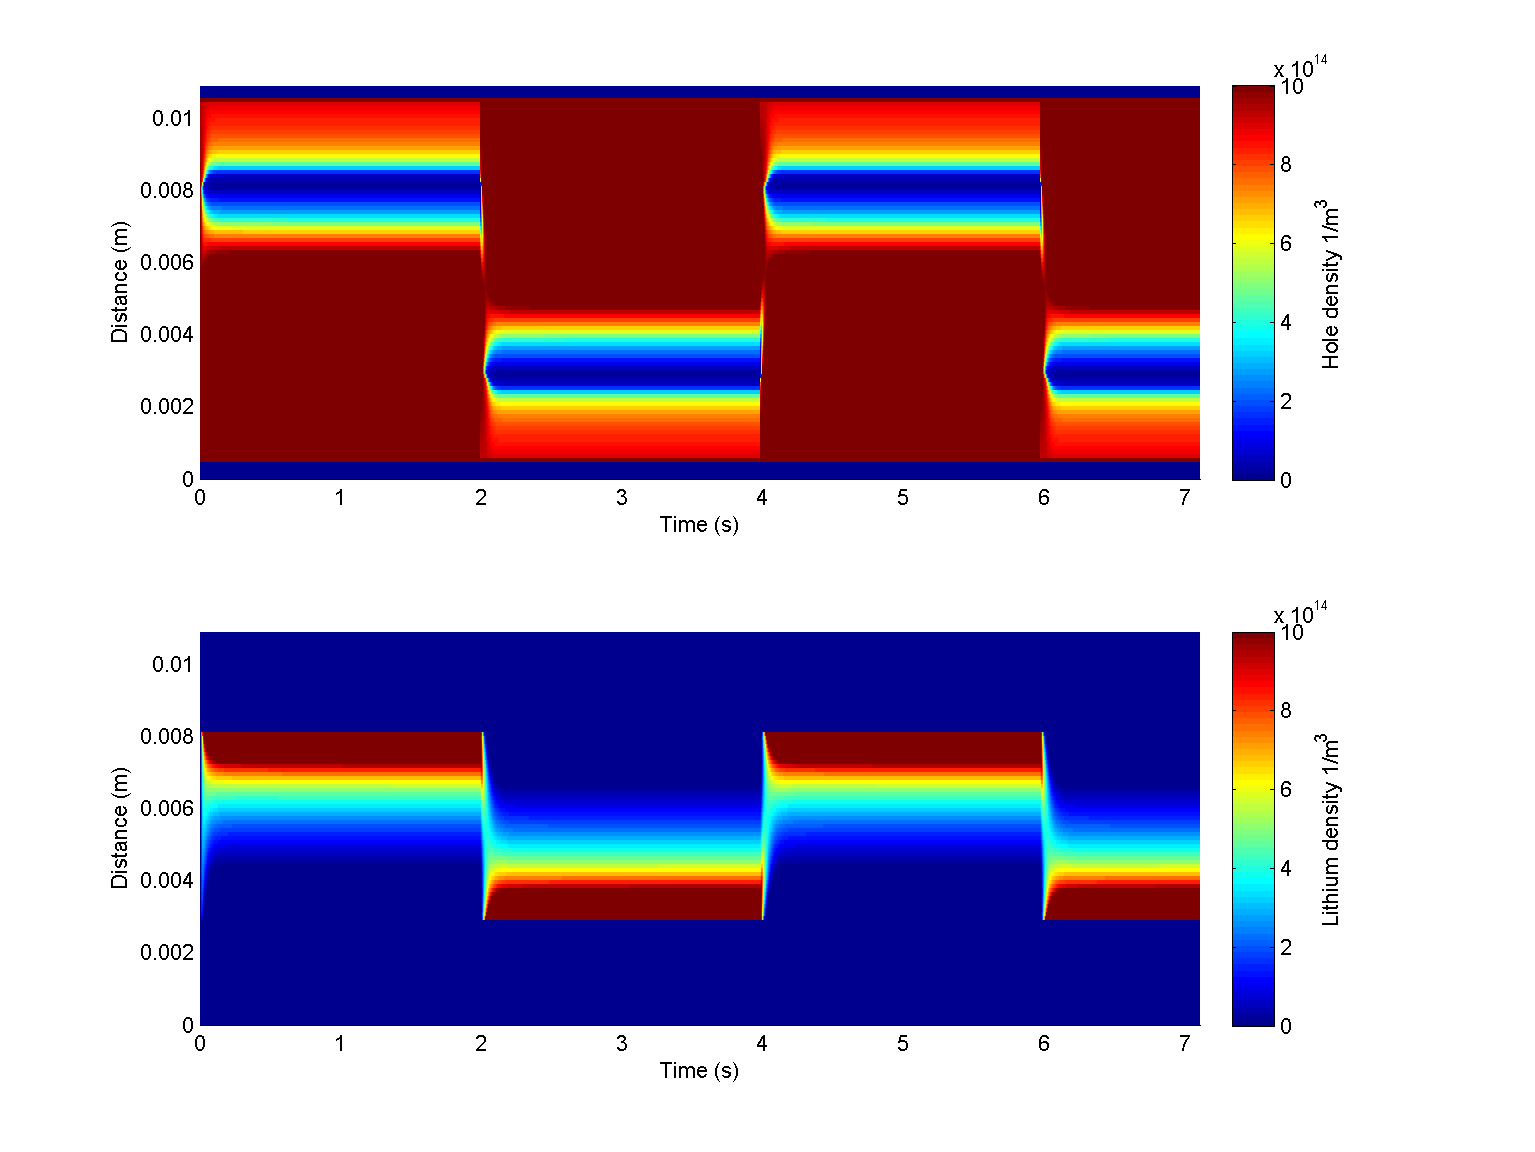
\includegraphics[scale=0.50]{2D_Memristor_Pulse_Lithium_Hole}
\caption{Lithium and hole density distributions over time} 
\label{lit_hole_dist}
\end{figure}


This final plot (figre \ref{mag_lit_curr}) shows the magnitude of the lithium current density over time. Almost all of the lithium ion movement occurs at the wet/dry interface of PEDOT:PSS since most of the electric field concentrates around that region. So when the potential is flipped from one side to the other, most of the lithium ions drift and diffuse back into the electrolyte instead of going through the PEDOT:PSS. This effect is also demonstrated in section 7.4 (figures \ref{notch} and \ref{Notch_flip_side}). 

\begin{figure}[!htp]
\centering
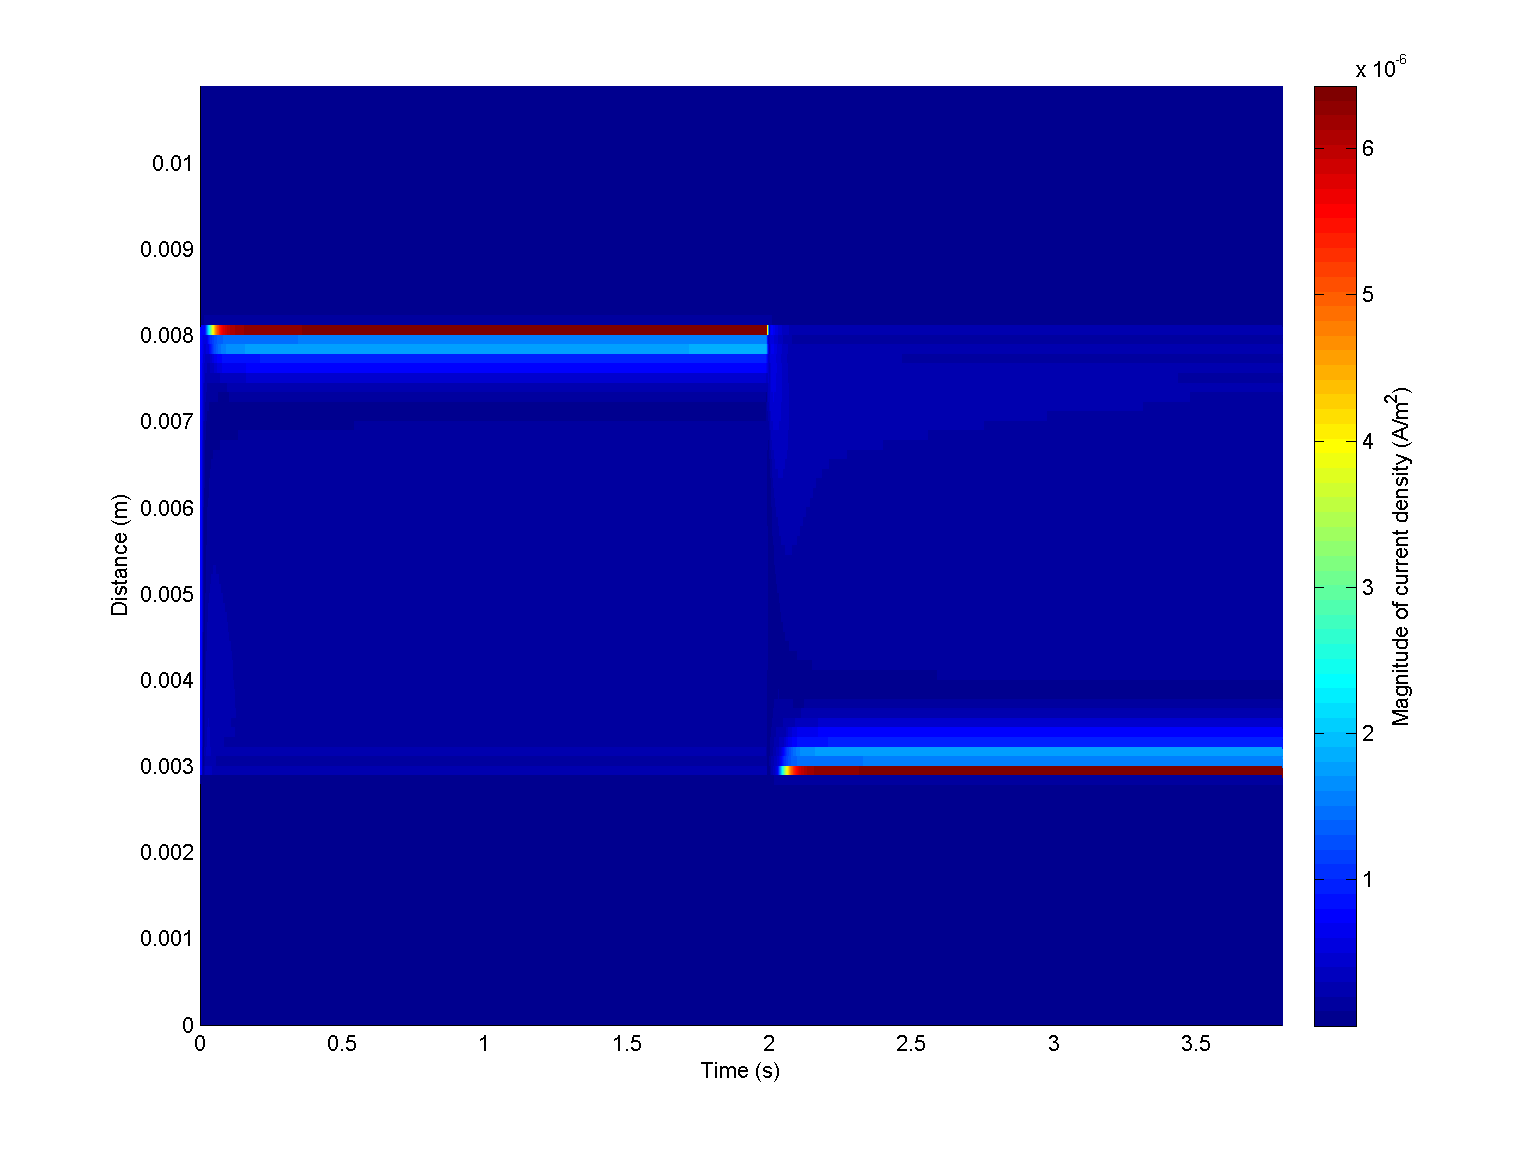
\includegraphics[scale=0.50]{2D_Memristor_Pulse_Lithium_J}
\caption{Lithium current density over time} 
\label{mag_lit_curr}
\end{figure}


\clearpage
\section{2-D Memristor Simulation Using a Sinusoid}

A memristor with an AC potential with different frequencies is simulated in this section. Following 4 plots (figure \ref{1dIV}) show the I-V curves of the memristor for 0.5, 5, 10 and 100 Hz. In these simulations there are two effects working against each other, the increase in the applied potential which increases the current output and the lithium ions working against the increase of the current by migrating into the PEDOT:PSS and increasing resistivity. Both of these effects can be clearly seen in the I-V curve for 0.5 Hz. Initially as the potential increases from 0 to 0.5 V, there is an increase in the current which means that there are not enough lithium ions in PEDOT:PSS to increase the resistivity of the device. As the potential reaches 0.5 V the accumulation of the lithium ions overtake the increase in potential such that the output current starts to decrease even though the potential is increasing. This effect disappears at higher frequencies since the lithium ions are too slow to catch up with the change in the potential. 
   
\begin{figure}[!htp]
\centering
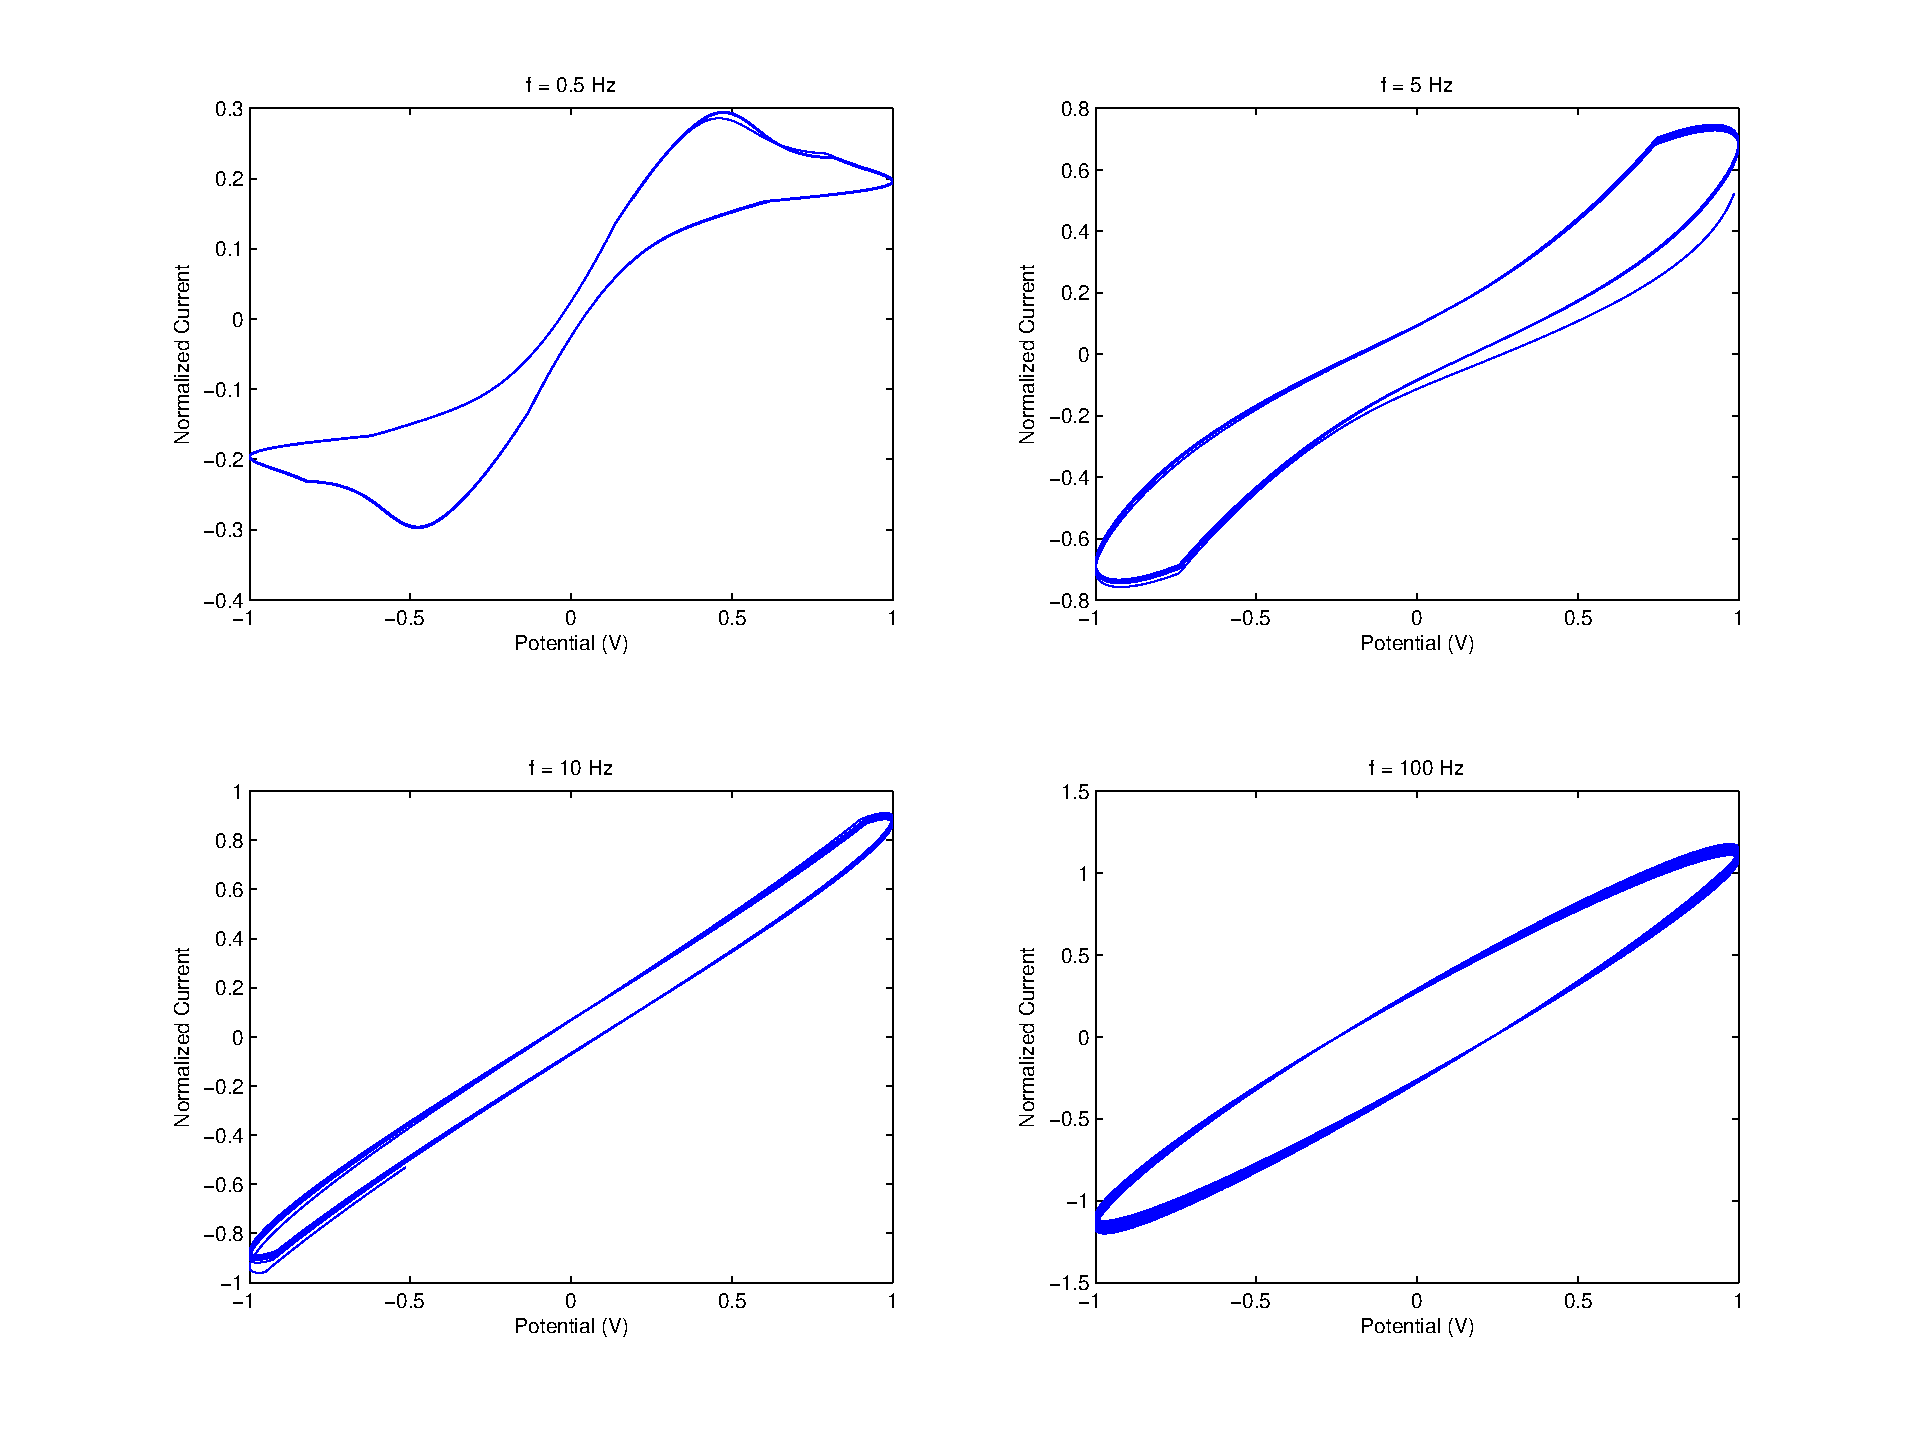
\includegraphics[scale=0.45]{2D_Memristor_bowtie_f}
\caption{Normalized Current vs. applied potential at different frequencies} 
\label{1dIV}
\end{figure}

There are a few differences between 1-D and 2-D simulations using AC potential which can be explained by using observations from the previous section. In 2-D simulations the resistivity measured from the left and the right contacts match each other quite closely. So the device current is symmetrical for both negative and positive potentials. 

During simulation, even though there is no applied potential, the current never goes to zero because of the stored electric field inside the PEDOT:PSS due to the accumulated charge. This capacitive effect prevents the current from going to zero when there is no applied potential. In 1-D simulations the amount of charge stored in the PEDOT:PSS is lower therefore the value of the current can get closer to zero compared to 2-D simulations.  

\begin{figure}[!htp]
\centering
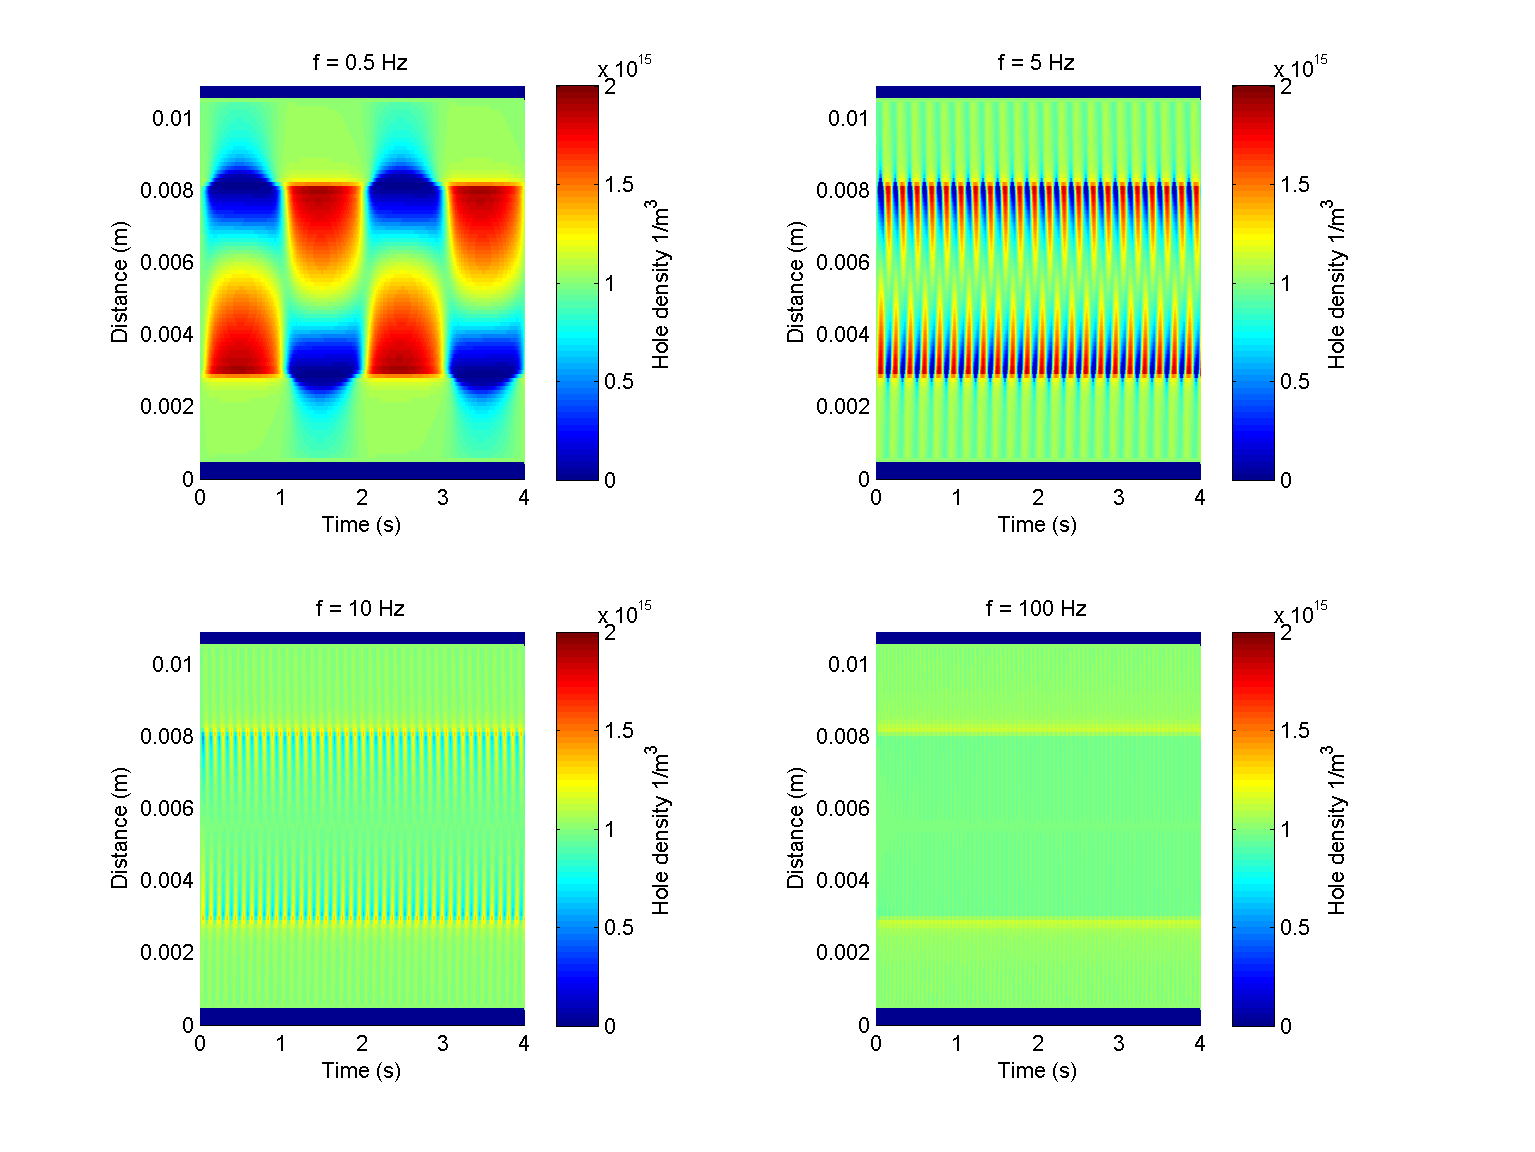
\includegraphics[scale=0.55]{2D_Memristor_f_Hole}
\caption{Hole distribution over time at different frequencies} 
\label{fhole}
\end{figure}

Figures \ref{fhole} and \ref{flit} show hole and lithium densities over time inside the PEDOT:PSS. At low frequencies the lack of holes due to the lithium ions as well as excess holes due to the perchlorate accumulation inside the electrolyte is clearly visible. At high frequencies, since the potential is changing rapidly, there is not enough time for the ions to accumulate on either side. So the hole distribution remains mostly undisturbed. \tjs{For  this case the} lithium ions move into the PEDOT:PSS only through diffusion \tjsr{but}{and} they do not affect the hole distribution. Based on these plots, it is possible to conclude that both 1-D and 2-D memristor models behave like a regular resistor at high frequencies. 


\begin{figure}[!htp]
\centering
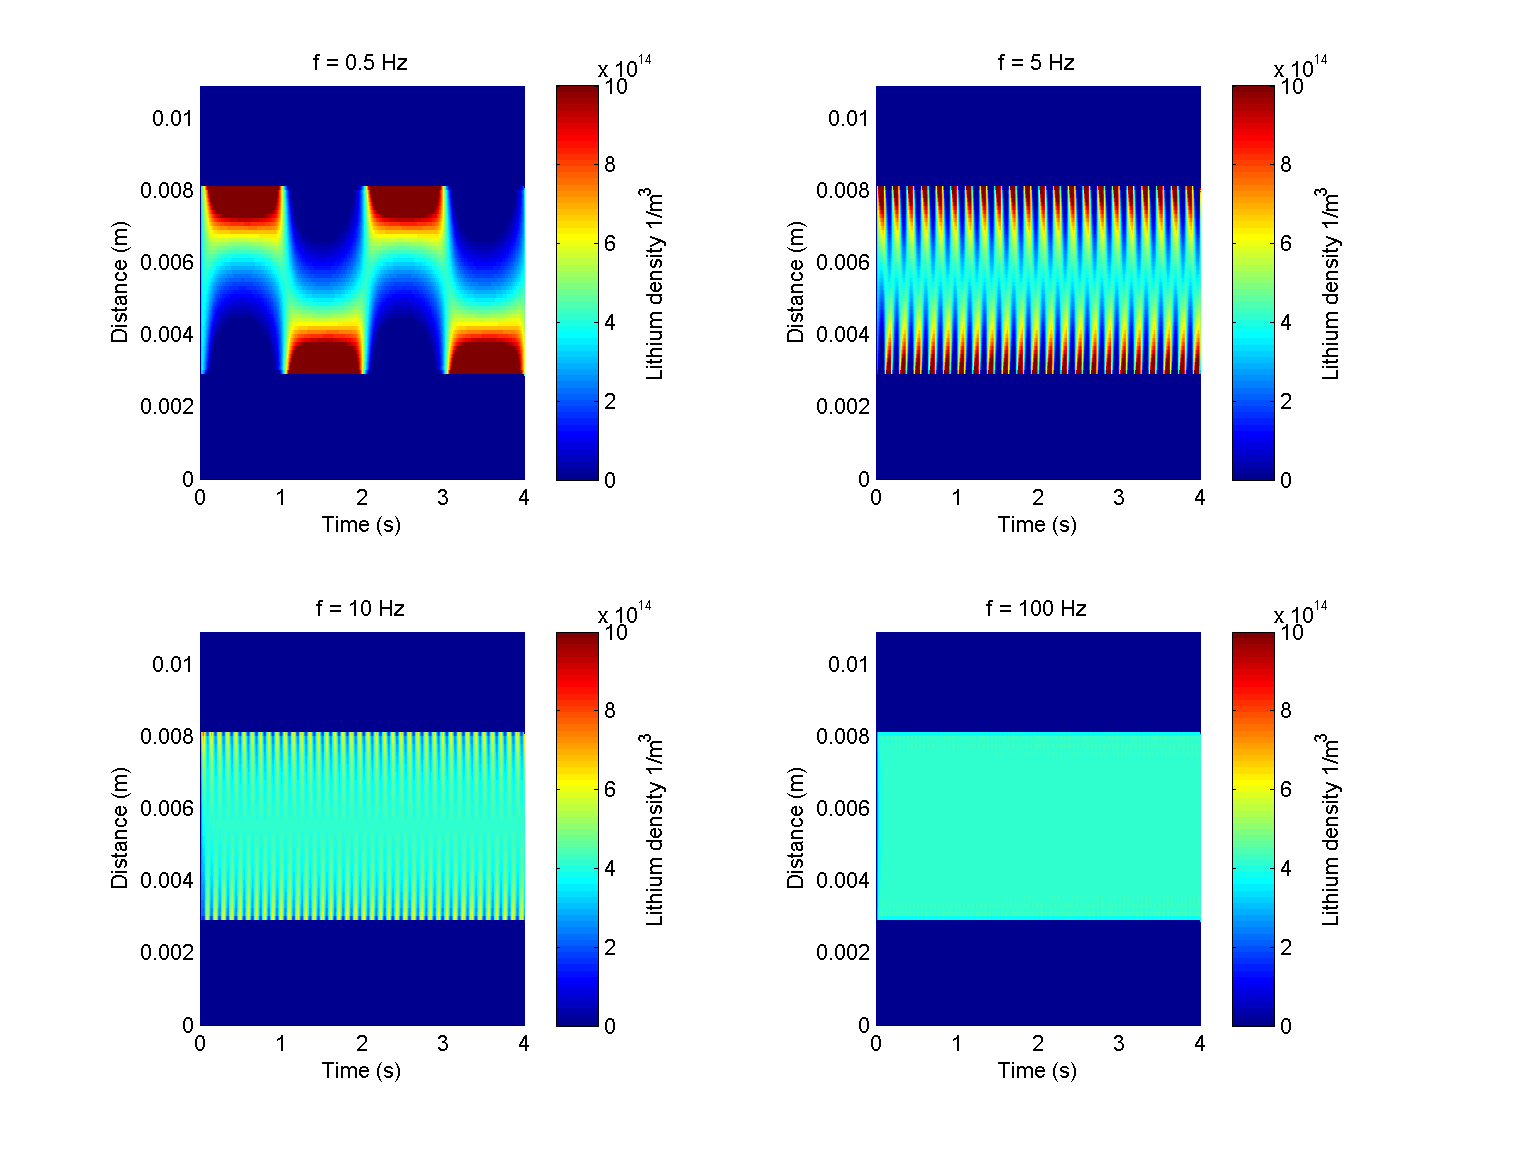
\includegraphics[scale=0.55]{2D_Memristor_f_Lithium}
\caption{Lithium distribution over time at different frequencies} 
\label{flit}
\end{figure}


\clearpage
\section{Experiment vs. Simulation}

The memristor model presented in this thesis has many approximations and it is far from complete but the preliminary simulations show promising results. In this section 2-D memristor simulations are compared with the experimental results in order to validate the model developed in this thesis. Due to the approximations and difficulties in the simulation mentioned in the previous chapters the current values obtained from the simulation are much lower than the actual device therefore the memristor model is only behaviorally compared to the experimental results. 


\begin{figure}[!htp]
\centering
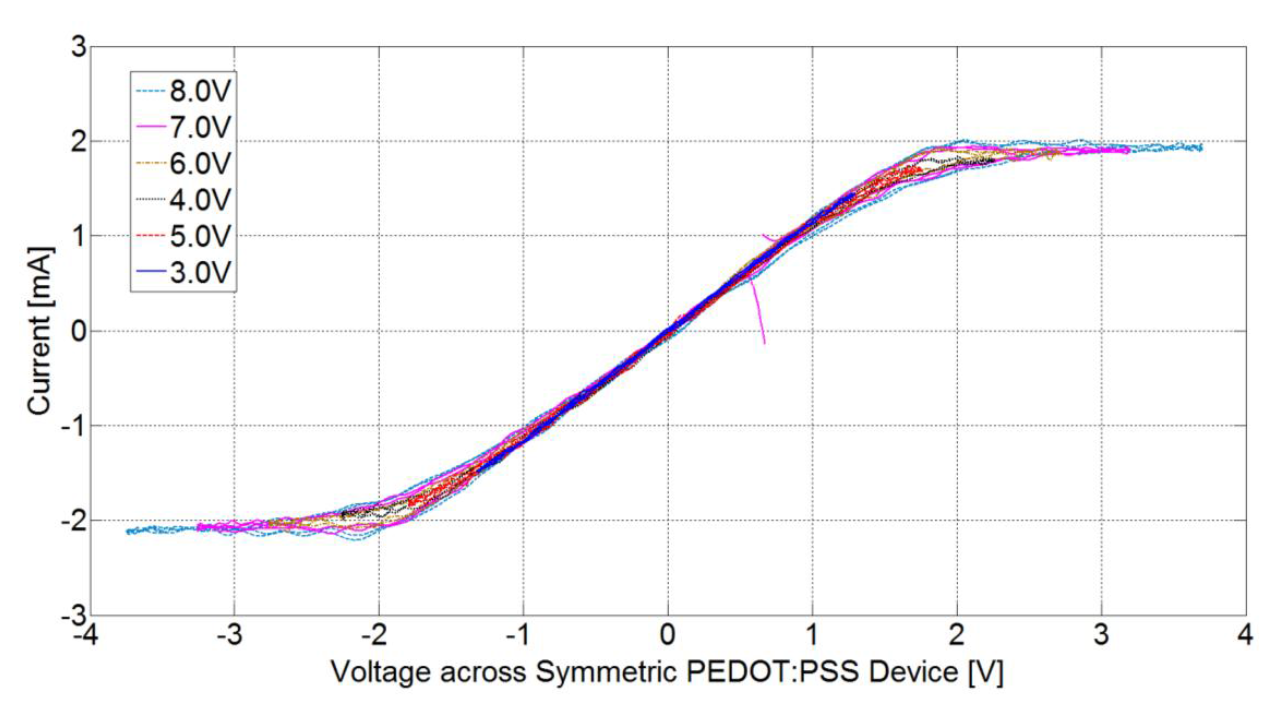
\includegraphics[scale=0.30]{memf1e-1}
\caption{Experimental results for various applied potentials at 0.1 Hz (Courtesy of Eduardo Barrera)\cite{eduardo}} 
\label{memf1e-1}
\end{figure}

\begin{figure}[!htp]
\centering
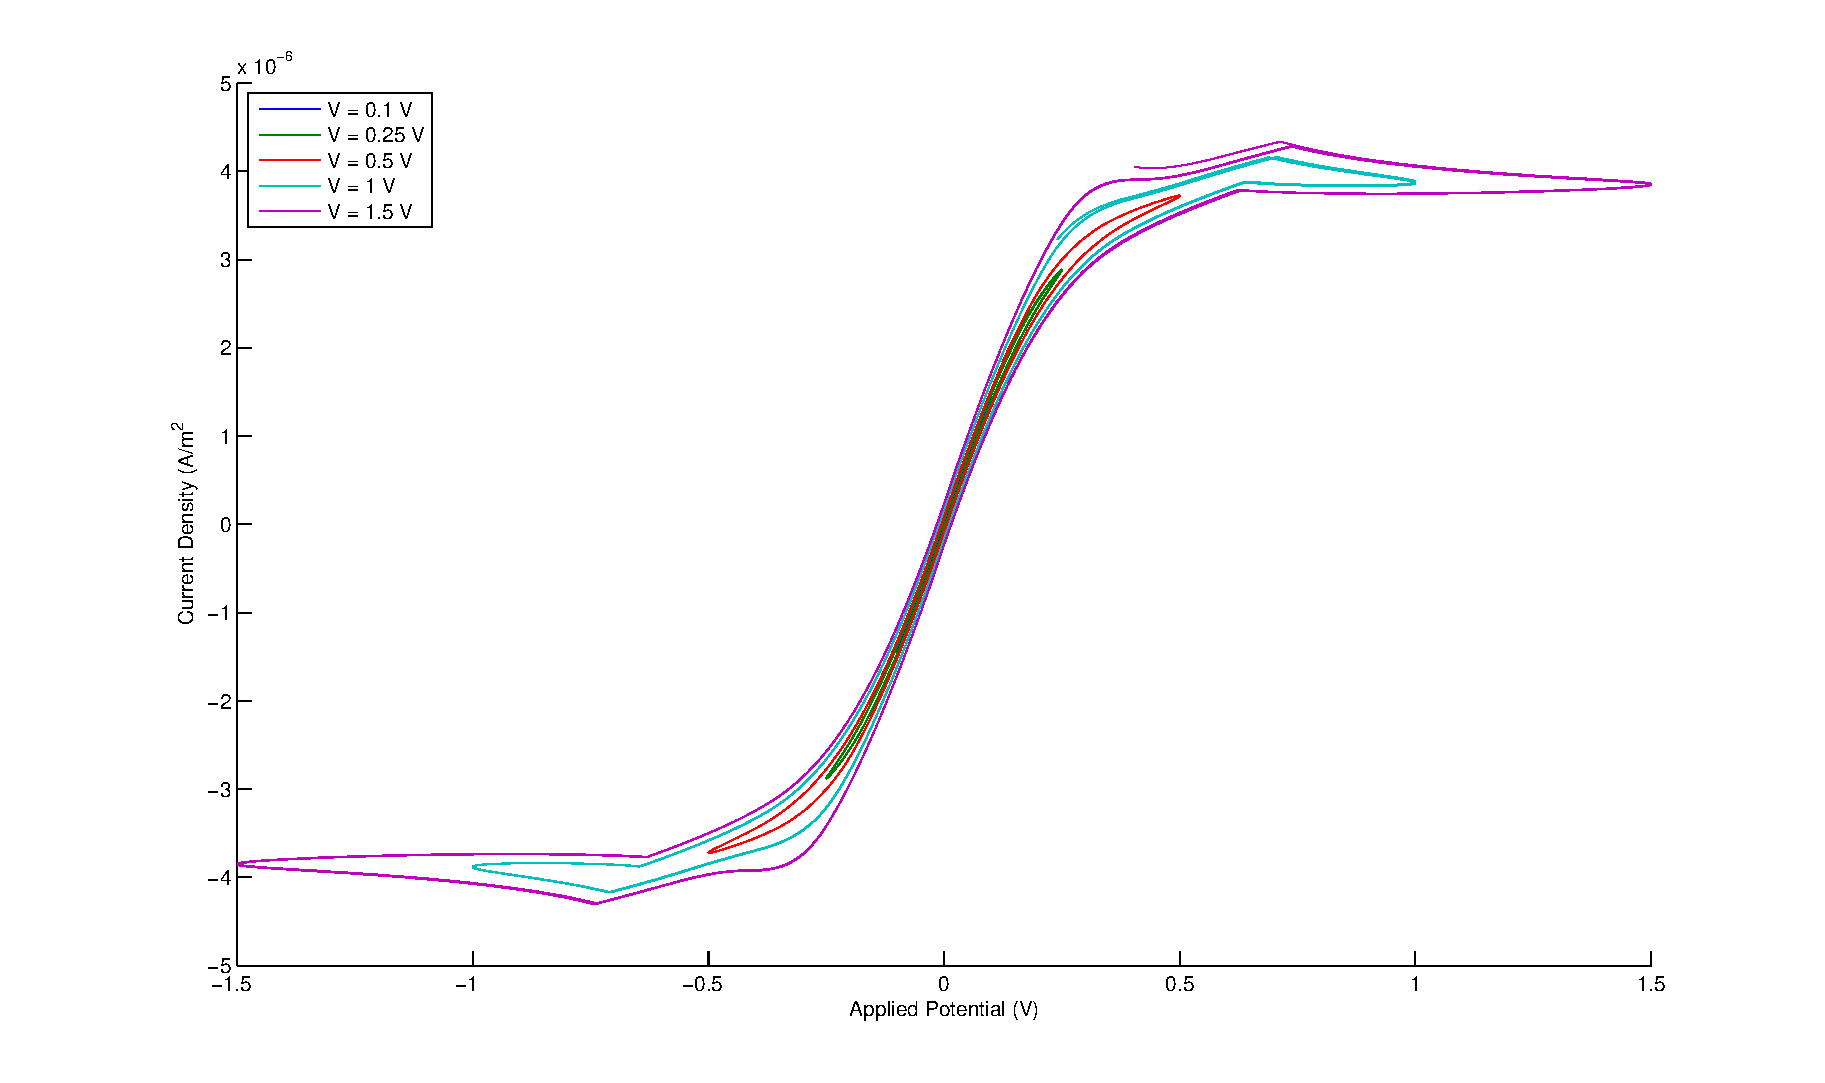
\includegraphics[scale=0.35]{Bowtief01Vchng}
\caption{Simulation results for various applied potentials at 0.1 Hz} 
\label{Bowtief01Vchng}
\end{figure}

Figures \ref{memf1e-1} and \ref{Bowtief01Vchng} show the I-V curve of the memristor using various potentials. At low potentials the current voltage relationship is linear for both simulation and experimental results which means that the resistance is constant over time. At low voltages lithium ions do not move very fast therefore the change in the resistivity of the PEDOT:PSS is minimal. At higher potentials the resistivity starts to increase due to the accumulation of the lithium ions and over time it completely cancels out the increase in the potential. 

\begin{figure}[!htp]
\centering
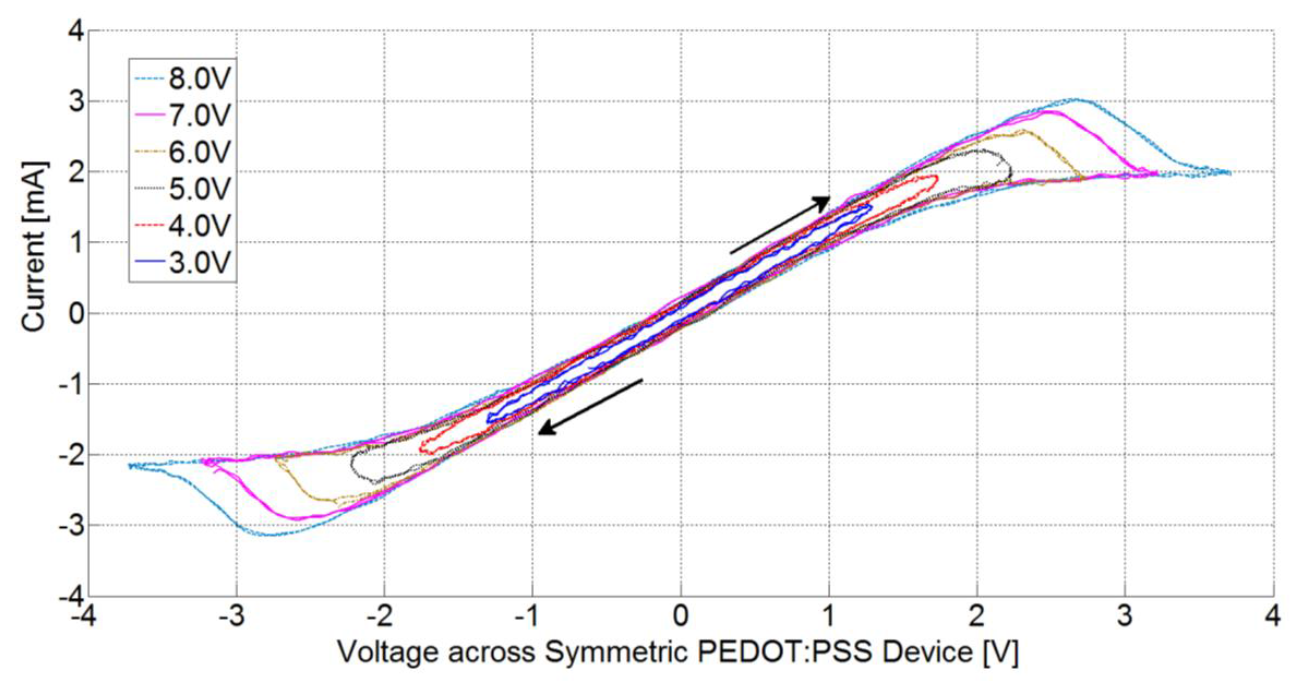
\includegraphics[scale=0.27]{memf1}
\caption{Experimental results for various applied potentials at 1.0 Hz (Courtesy of Eduardo Barrera)\cite{eduardo}} 
\label{memf1}
\end{figure}

For the plots \ref{memf1} and \ref{2D_Memristor_5e-1Hz} the same experiment is repeated using a frequency of 1.0 Hz. This time the linear region is longer since the change in potential is faster and lithium ions cannot keep up with it. Once the movement of the lithium ions speeds up due to the applied potential and there is enough accumulation inside the PEDOT:PSS then the resistivity increases much faster than the increase in the potential. 

\begin{figure}[!htp]
\centering
% 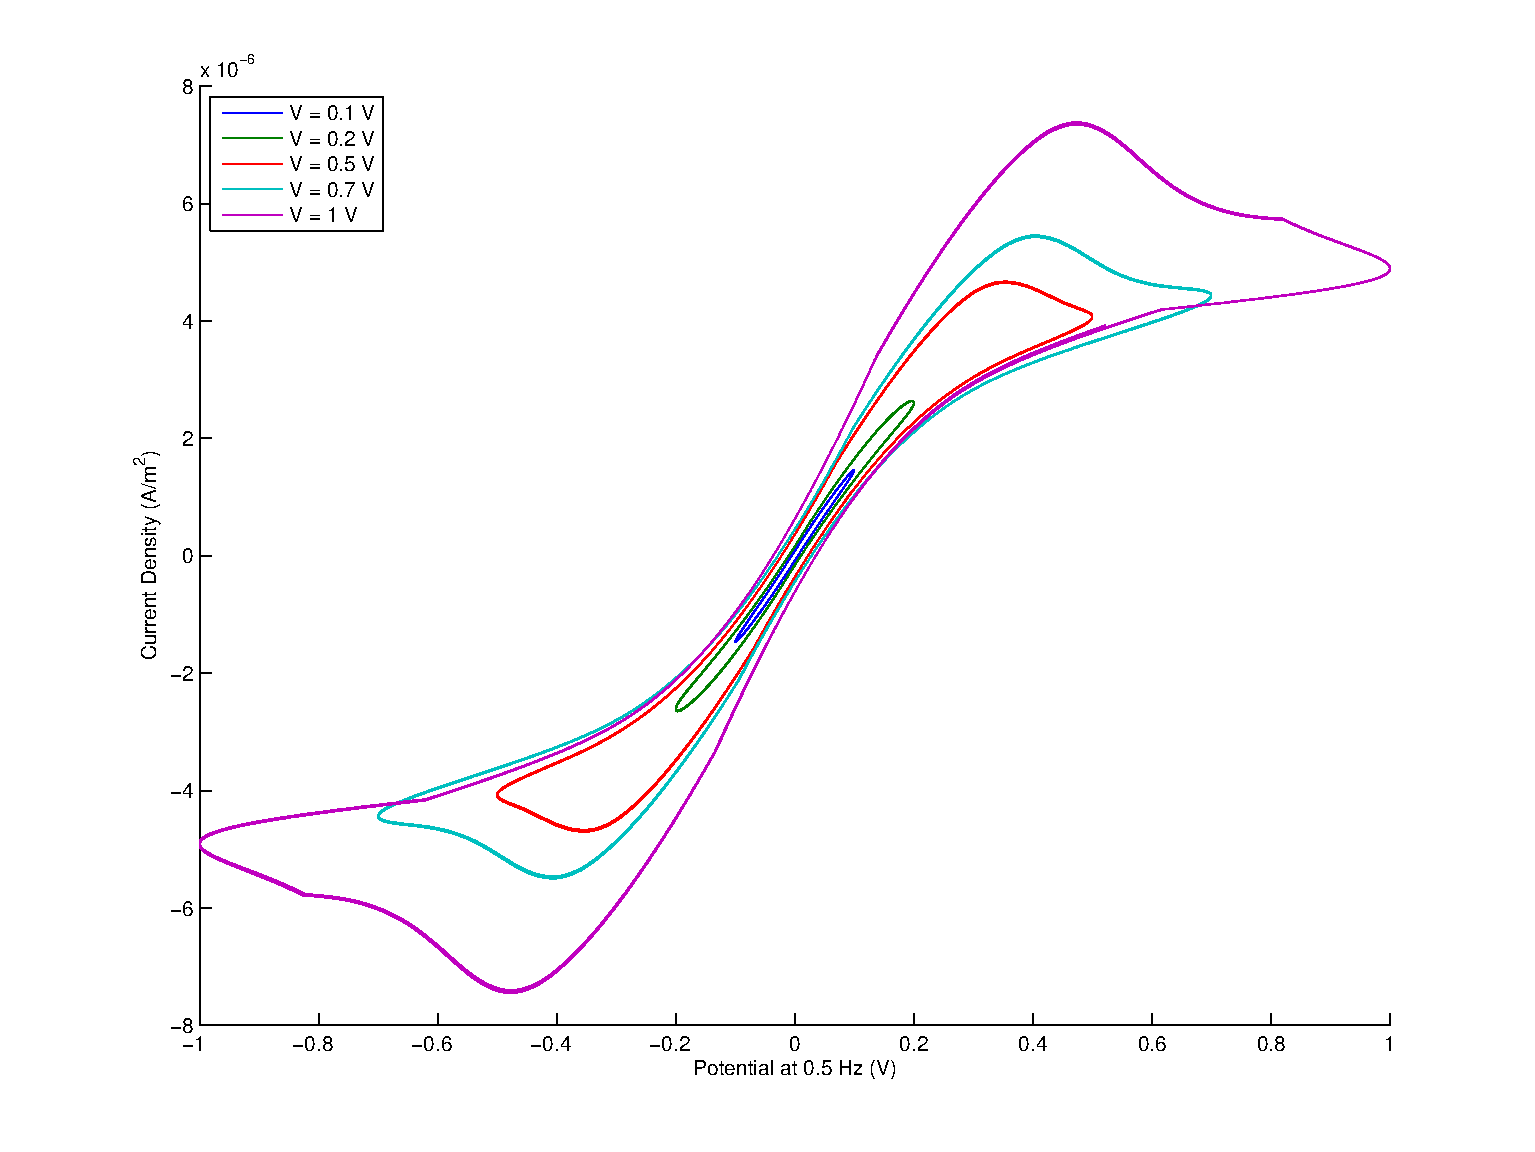
\includegraphics[scale=0.35]{2D_Memristor_5e-1Hz}
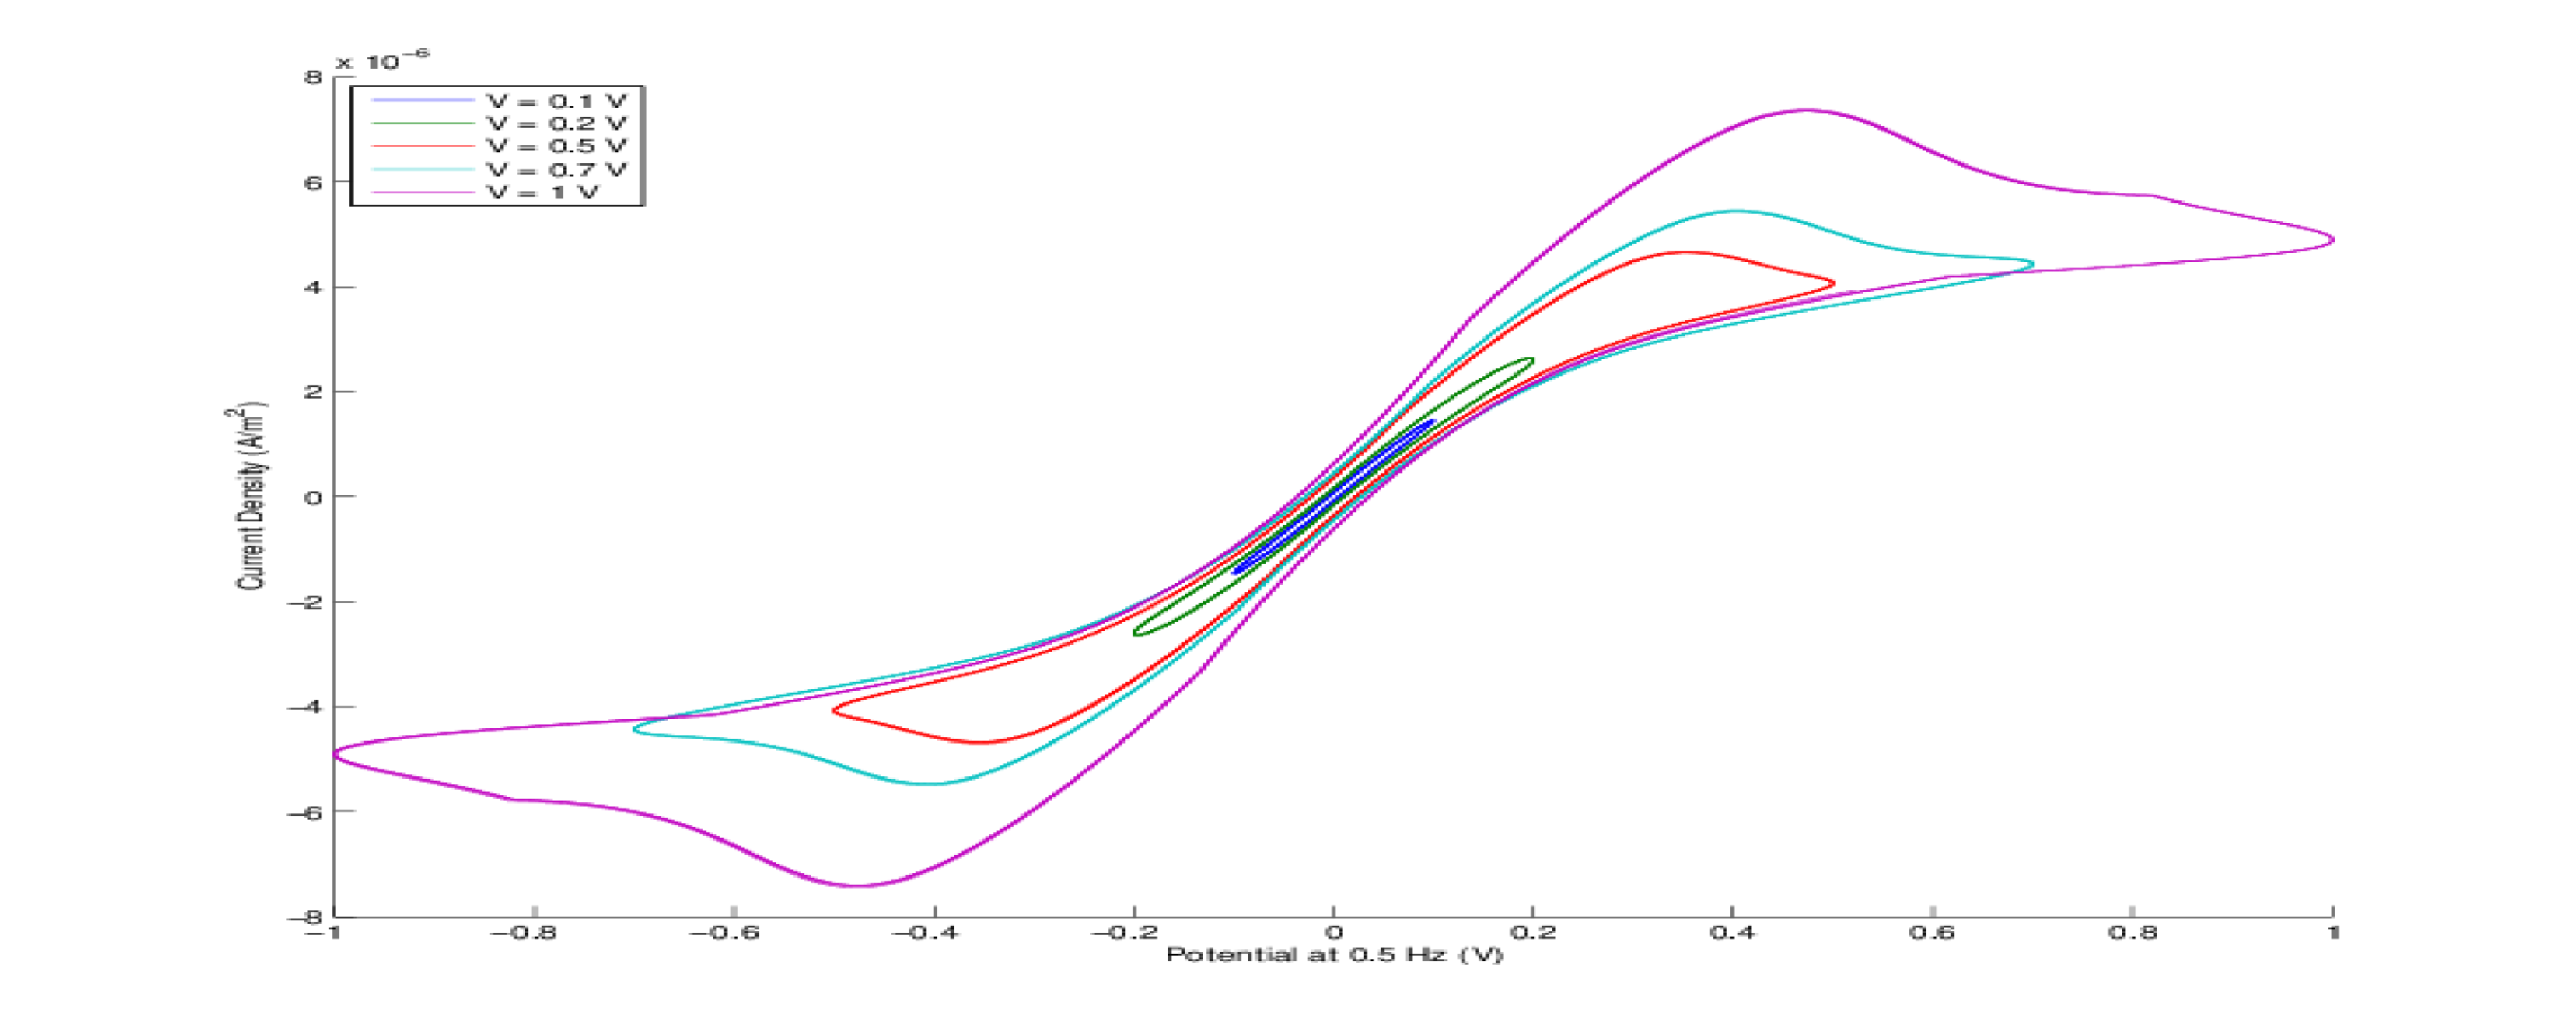
\includegraphics[scale=0.125]{2D_Memristor_5e-1Hz-2}
\caption{Simulation results for various applied potentials at 1.0 Hz \tjs{tjs scaled plot}} 
\label{2D_Memristor_5e-1Hz}
\end{figure}

The pinched area towards the end of the outermost loop shows that the change in resistivity slows down as it starts to reach its maximum value. This is also apparent in the transient simulations with a potential pulse train. The increase in resistance is fast up to a certain value and then it slows down as PEDOT:PSS is saturated by lithium ions.

The following plots (\ref{experimental} and \ref{MemF}) are created using a variable frequency instead of a variable potential. For the simulation and the experiment, the memristor behaves more like a resistor as frequency increases. This is due to lithium ions not having enough time to drift into the PEDOT:PSS to make a change in the resistance. Even though the frequencies used for simulation \tjsr{is}{are} different than the ones used in the experiment, both plots show similar behavior. A better match can \tjs{likely} be achieved by improving the mobility models used for lithium ions and holes. 

\begin{figure}[!htp]
\centering
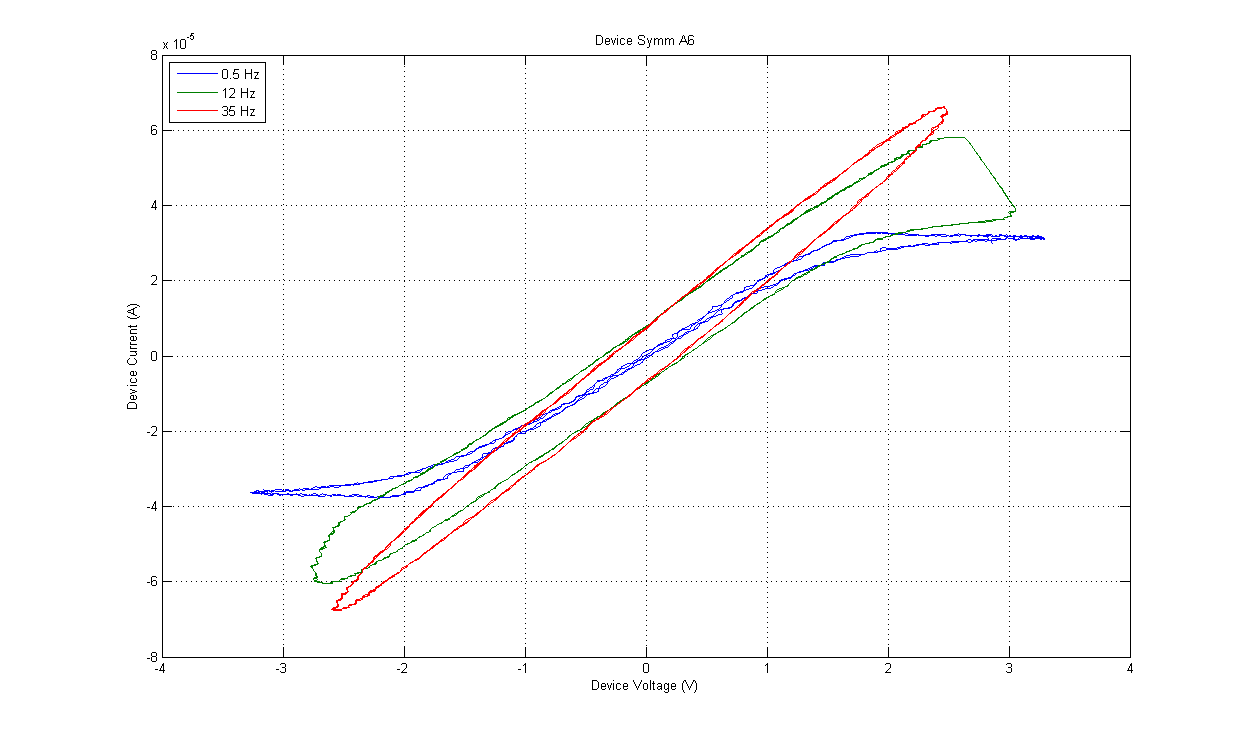
\includegraphics[scale=0.31]{experimental}
\caption{Measured I-V curve at different frequencies (Courtesy of Eduardo Barrera)\cite{eduardo}} 
\label{experimental}
\end{figure}

\begin{figure}[!htp]
\centering
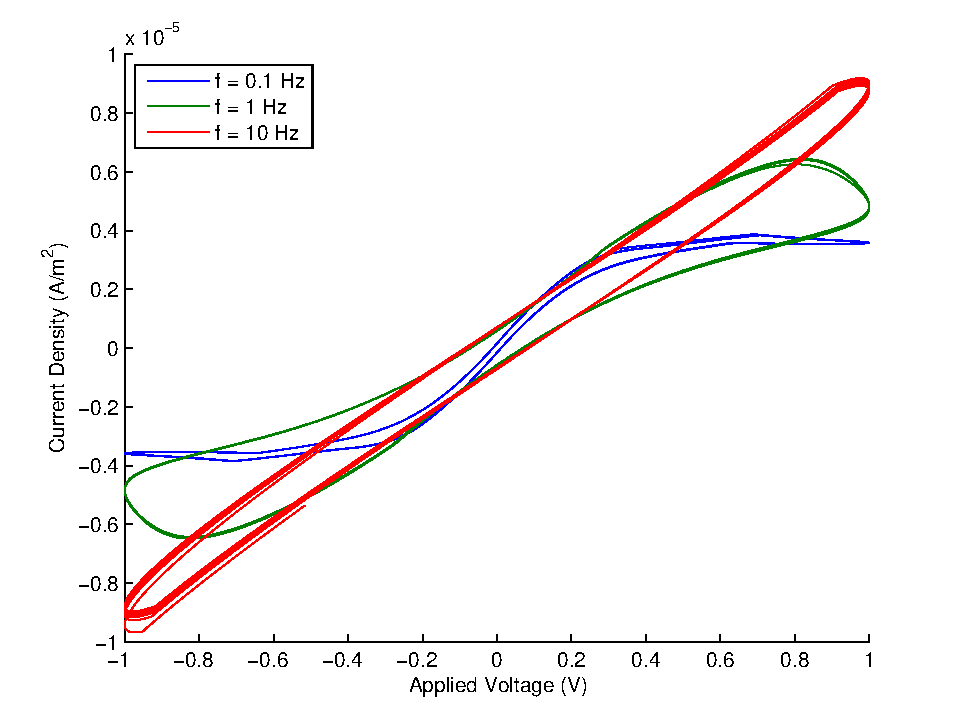
\includegraphics[scale=0.55]{MemF}
\caption{Simulated I-V curve at different frequencies } 
\label{MemF}
\end{figure}

\clearpage
This last example consists of a memristor where PEDOT:PSS strip is separated into two pieces with a notch which prohibits the hole flow trough the device. Figure \ref{notch} shows the measured movement of lithium from the right strip to the left strip. Red color represents the lack of charge and blue color shows the presence of charge. For the simulation results (figre \ref{Notch_flip_side}) red color represents a high charge density and blue color represents a low charge density.

\begin{figure}[!htp]
\centering
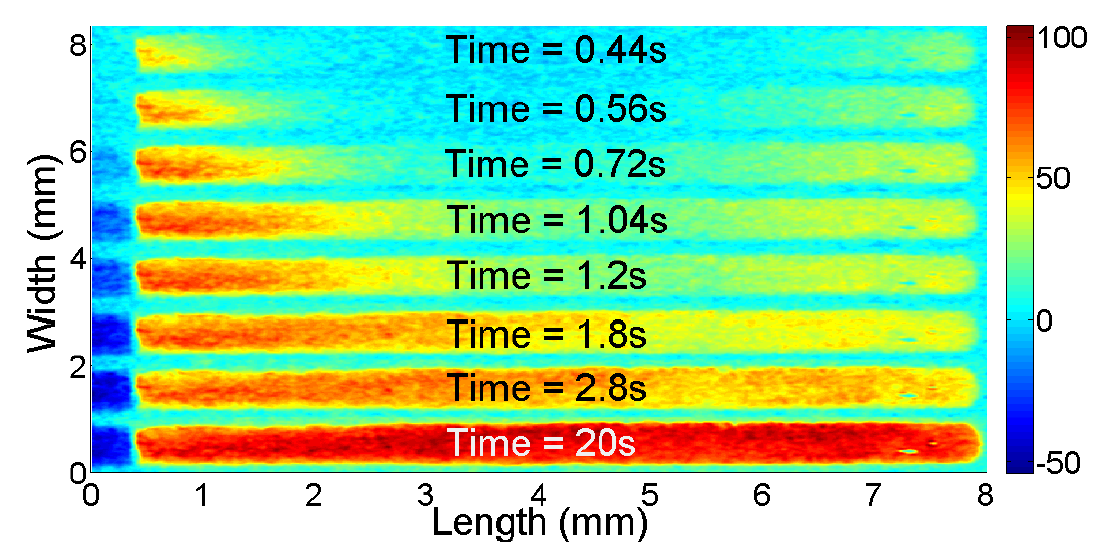
\includegraphics[scale=0.45]{notch}
\caption{Experimental results for accumulation of lithium inside PEDOT:PSS (Courtesy of Eduardo Barrera)} 
\label{notch}
\end{figure}

\begin{figure}[!htp]
\centering
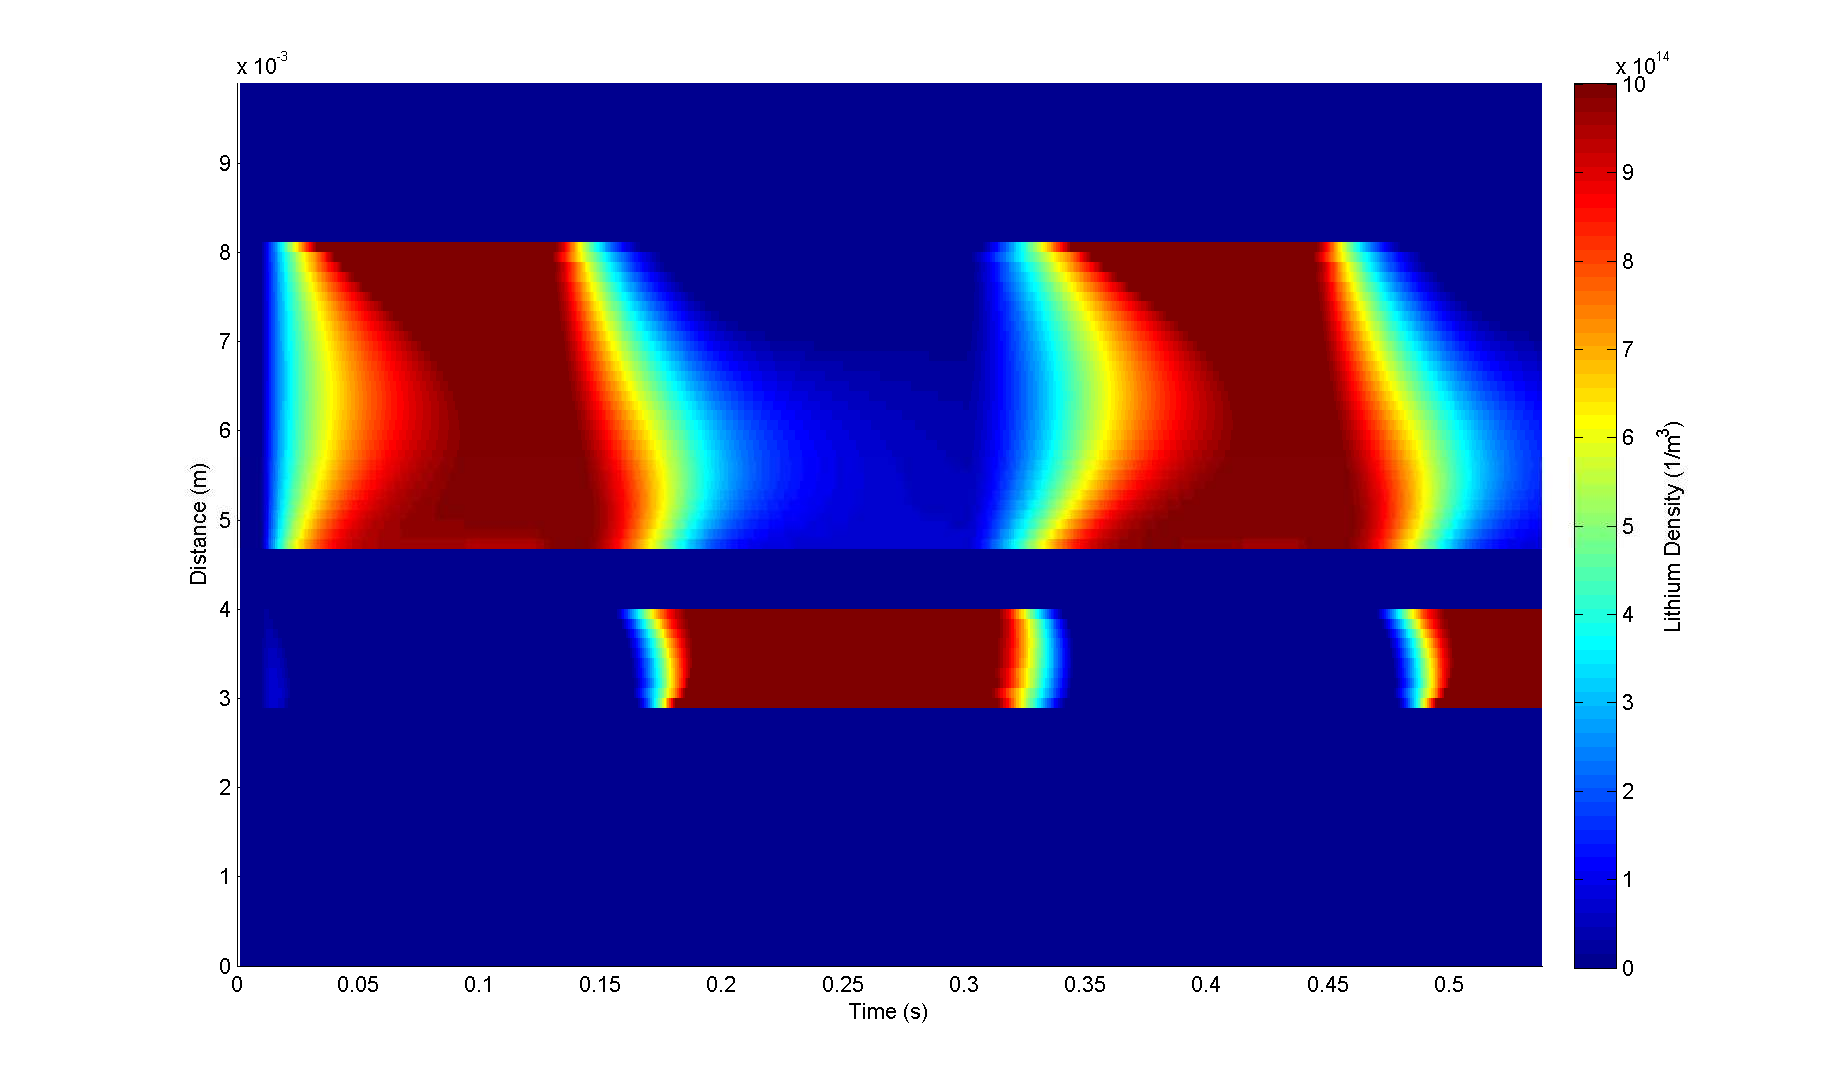
\includegraphics[scale=0.45]{Notch_flip_side}
\caption{Simulation results for accumulation of lithium inside PEDOT:PSS \tjs{[Ok I'm having trouble with the comparison]}} 
\label{Notch_flip_side}
\end{figure}

When a potential is applied, one side of the PEDOT:PSS strip is filled with lithium ions. It can be seen from both the simulation and the experimental results that the lithium ions start migrate out of the PEDOT:PSS near the notch and the wet/dry PEDOT:PSS interface which are the areas with highest electric field. Both plots show that lithium ions uniformly distribute themselves inside PEDOT:PSS at steady state. This uniform distribution of lithium ions supports the assumption that there is a limit on how many lithium ions PEDOT:PSS can accept per unit area. If this was not the case the lithium ions would have accumulated on one side of the device instead of being uniformly distributed.


\end{doublespace}

